%
% Main LaTeX file [referred to as the $(MAINFILE).tex in the Makefile] 
% to be used as template for writing MS thesis / PhD dissertation 
% at Michigan Technological University, Houghton, MI
%
%


% Document type
% Uncomment the line below for single sided printing 
% \documentclass[letterpaper,12pt,fleqn]{report}
\documentclass[letterpaper,twoside,12pt,fleqn]{report}

% Necessary packages
% MichiganTech_MSPhD.sty 
% This will in turn load all other required packages and (re)define
% several aspects to make the document compliant with Michigan Tech
% Graduate School requirements
%\usepackage{MichiganTech_MSPhD}
%\usepackage{mtustyle}
\usepackage{citelist}
\usepackage{hepparticles}


% Information required for Title & Signature pages
%% University
\university{HUMBOLDT UNIVERSITY}
%% Thesis/Dissertation title
\thesistitle{A Search for Extended Gamma-ray Emission from the Galactic Center with VERITAS}
%% Thesis/Dissertation author
\thesisauthor{Nathan C. Kelley-Hoskins}
%% Thesis/Dissertation year
\thesisyear{2015}
%% Department or School
\deptschool{Physics}
%% Program (optional)
\program{Physics}
%% Chair of the primary/home department
%% \deptchair{} must be empty, if \schooldean is not empty
\deptchair{???}
%% Dean of the School - applies if you entered a school for \dept{}
%% \schooldean{} must be empty, if \deptchair is not empty
\schooldean{}
%% Primary advisor
\primaryadvisor{Dr. Gernot Maier}
%% Co-Advisor (optional)
\coadvisor{}
%% Advisory committee member #1 (optional)
\advcommone{???}
%% Advisory committee member #2 (optional)
\advcommtwo{???}
%% Advisory committee member #3 (optional)
\advcommthree{???}
%% Advisory committee member #4 (optional)
\advcommfour{Dr. Advisory Committee \#4}


% Document begins
\begin{document}

% Allow very (though not arbitrarily) bad line spacing
% Ignore lines overfull by less than half a point (less than 2/10th of a mm)
% Add an extra 3 em of stretchability to each line
\sloppy

% Begin roman page numbering and empty page style
\pagenumbering{roman}
\pagestyle{empty}

% Title and Signature pages
%% For MS: replace \phdtitlepage with \mstitlepage
%%         replace \phdsignaturepage with \mssignaturepage
\phdtitlepage
%\mstitlepage
\cleartooddpage[\thispagestyle{empty}]
\phdsignaturepage
%\mssignaturepage

% Modular segments
\setstretch{2.0}
\pagestyle{plain} 

%% Dedication (optional)
%\include{Dedication}

%% Table of Contents (ToC), List of Figures (LoF) and List  of Tables (LoT) 
% Table of Contents
\cleartooddpage[\thispagestyle{empty}]
\currentpdfbookmark{Contents}{Contents}
\tableofcontents

% List of Figures
\cleartooddpage[\thispagestyle{plain}]
\listoffigures

% List of Tables
\cleartooddpage[\thispagestyle{plain}]
\listoftables


%% Preface (optional)
% \include{Preface}

%% Acknowledgments
%\include{Acknowledgments}

%% Abstract
\cleartooddpage[\thispagestyle{empty}]
\phantomsection
\section*{Abstract}
\addcontentsline{toc}{chapter}{Abstract}

VERITAS is a Gamma-Ray Observatory that has been observing astrophysical gamma-ray targets like the Galactic Center for several years.
As VERITAS is in the Northern Hemisphere, this means the telescope detects Gamma Rays at a low elevation.
This leads to the telescope being sensitive to higher energy gamma rays than if it were pointed directly overhead.
As the Galactic Center is at low elevations and is a prime target for Dark Matter searches, a probe of Dark Matter at unsearched energies is possible.
This dissertation presents the analysis methods used to search for Dark Matter near the Galactic Center from gamma rays with energies between 4 and 70 TeV.

{\color{red}(need to expand, one page??)}

%% add a blank page for margin styling
%\newpage
%\null
%\thispagestyle{empty}
%\newpage

\cleartoevenpage[\thispagestyle{plain}]
\null


%% Begin arabic page numbering
\pagenumbering{arabic}

%% Chapters
\cleartooddpage[\thispagestyle{empty}]
\chapter{Introduction}


\section{Dark Matter}

\section{Galactic Center}

\section{Gamma-Ray Astronomy}

\section{Science Objectives}

\section{Gamma-Ray Showers}
\section{Gamma Ray Detectors}

Veritas

Veritas is a gamma-ray observatory.
This observatory consists of 4 telescopes, spread out over an area of 50 meters.
Each telescope consists of a 12m dish of 498 mirrors, with a customized 498 pixel single-photon timing camera at the end of a 7 meter boom.

Gamma rays are reconstructed and observed through a multi-stage process.
First, gamma rays are emitted from an astrophysical source, outside the solar system.
Then, these gamma rays travel to Earth and interact with molecules of Earth's atmosphere.
When they interact, they pair-produce into an electron-positron pair, where each has an energy of half the parent gamma ray.
The positron will then annihilate with an atmospheric electron, producing 2 more gamma rays, while the electron will shed some energy through ionization and by emitting chernekov photons.

This process will repeat over and over, creating a particle shower, until the electrons have ~80MeV of kinetic energy, at which point ionization will dominate the energy loss, and the shower will stop producing cherenkov light.

Veritas telescopes are designed to detect the cherenkov photons emitted from these particle showers, timing their arrival in each pixel to within 1 nanosecond.
The shower images produces by multiple telescopes can then be used to triangulate the original gamma ray's point of orgiin, whereas the size of the shower can be used to determine the gamma ray's energy.


Effective Area
For the calculation of the flux, the detection area must be found.
This depends primarily on each gamma ray's energy, as well as its detected position in the camera.


\cleartooddpage[\thispagestyle{empty}]
\chapter{Dark Matter}

\section{Evidence for Dark Matter}

Peering out into space, there is evidence for dark matter on several different length scales.
As this dark matter, by definition does not interact with light in any significant way, most of the evidence for dark matter relies on a combination of gravtiational and optical observations.

% 10^19m comes from: 
% fornax dwarf spheroidal galaxy wiki page
%    17' x 12.6' in solid angle, call it 15'
%    140kpc away  
%    140kpc * Tan(15') = 0.6kpc = 1.8*10^19m ~ 10^19m
At the smallest scale of $\nicetilde 10^{19}$m, groups of several thousand stars can be seen revolving around a center of mass, at a larger spread of speeds than allowed by the existing visible amount of matter.
%
% galaxy rotation curve wiki page, M33 has curve measurements out to 50,000ly
%   50,000ly = 4.7*10^20m ~ 10^20m
At galactic scales of $\nicetilde 10^{20}$m, the light from stars, as well as hydrogen lines, can be used to measure the amount of mass and its rotational velocity around the center of galaxies.
%
% galaxy cluster wiki page
% 2-10 Mpc, call it 6Mpc = 1.85*10^23m ~ 10^23m
At cluster scales of $\nicetilde 10^{23}$m, galaxy velocities can be measured and compared, x-ray telescopes can monitor the amount of hot gas, and mass-heavy areas of space will gravitationally lens background galaxies.
%
% age of universe (13.82*10^9 years * speed of light) = 1.307*10^26m
At the universe scale of $\nicetilde 10^{26}$m, the measurement of oscillations in the dipole spectrum of the cosmic microwave background can be used to determine the amount of dark matter.


\subsection{Dwarf Galaxy Scale}
At the smallest scale, satellite galaxies consist of several thousand, individually-resolvable stars.
Telescopes can measure the spectra of these stars, allowing for their velocity to be calculated.
By looking at how fast each star is moving around the satellite galaxy's center of mass, and how widely these rotational velocities differ, the amount of enclosed mass can be inferred.

\subsection{Galaxy Scale}
At the next highest scale, the total amount of light produced by a quadrant of a galaxy is measured with telescopes.
Known mass-to-light ratios can then be used to calculate the total amount of mass within that quadrant.
This was the earliest method of measuring the mass of a galaxy, producing a low calculation for the amount of mass.

xray gas??

In the third method, a galaxy's emission spectrum is observed at many positions around its structure (center, outer edges, etc).
By comparing the orientation of the disk with the doppler-shifted position of common spectral lines, one can calculate the average velocity that each chunk is travelling at around the center of the galaxy.
Newton's law of gravity can then be used to calculate the mass contained within a sphere of that same radius.
This calculation ends up with a larger amount of mass.

\subsection{Galaxy Cluster Scale}
In the fourth method, a large swath of space can be observed with high-resolution telescopes.
Volumes of space with large amounts of matter will bend the light from background galaxies in known ways.
By examining how the images of different background galaxies are bent, the amount of mass between the galaxy and the observer can be inferred.
This is typically used for measuring the mass of cluster-sized volumes of space, rather than individual galaxies.

\subsection{Universe Scale}
At the largest scale, the cosmic microwave background (CMB) has been used to measure the total amount of dark matter in the universe.
By looking at the structure of the CMB, earlier times in the universe can be studied.
Closer to the big bang, there was a point in time referred to as the 'freezout'.
Before that time, the universe was a sea of quark plasma and other particles, and the temperature was too hot to allow baryons exist for any long period of time.
After that freezout time, the temperature had dropped to the point where more baryons were created than destroyed, much like cooling steam condensing to liquid water.
This freezout left an imprint of its structure, more CMB photons in some places, less in others.
By looking at this CMB structure, the total number of baryons in the universe can be measured.
??Volume measured??



\section{Old}

Dark matter was named as a solution to an inconsitancy in galactic rotation curves.

Hydrogen spectral lines were studied from various places in different galaxies.
From these spectral lines, doppler shifts could be used to calculate the radial velocity of that area of the galaxy.
By comparing the radial velocities at different distances from the visible center of galaxies, a profile can be created that charts the enclosed mass.

Alternately, star formation can be simulated, which can be used to predict the amount of light seen for each solar mass in a region.
From this second method, the mass contained in a galaxy can also be measured at each radial distance from the galaxy's center.

By comparing these two mass curves, it has been found that they differ greatly.
Thus, the concept of dark matter was invented to make up for the discrepancy between these two curves.

% core profile

% einasto


Dark Matter is viewed as the seed for where galaxy clusters form in the universe.


Due to how the universe formed, the missing matter is not percieved to be locked up in baryons.

% discuss how cosmology rules out

\section{The Standard Model}

WIMPs
Axions
???

\section{Particle Accelerators}

Supernova remnants, Pulsar Wind Nebulae, any kind of jet


\section{Search Techniques}

There are three general methods of search for dark matter particles.
Direct Detection experiments attempt to discern when a dark matter particle directly strikes a volume of detection mass, stored deep underground.
Indirect Detection experiments attempt to look for secondary products of dark matter interactions, usually through astrophysical searchs.
Collider searches attempt to produce a dark matter particle through controlled collisions of standard model particles.

\subsection{Direct Searches}

\subsection{Indirect Searches}

\subsection{Collider Searches}

% direct
% indirect
% collider


\section{Mass and Cross-section}



\cleartooddpage[\thispagestyle{empty}]

\newcommand{\Lim}[1]{\raisebox{0.5ex}{\scalebox{0.8}{$\displaystyle \lim_{#1}\;$}}}
\renewcommand{\labelitemi}{\textbullet}

\chapter{Gamma Rays and Dark Matter}\label{ch_gamma}


This analysis searches for dark matter using gamma rays, thus a discussion on gamma rays and their properties is necessary.
In this chapter, three different topics are discussed.
The first is the astrophysical mechanisms that produce gamma rays, the second is how dark matter around the Galactic Center can produce gamma rays, and the third is how gamma rays induce air showers in the Earth's atmosphere.

\section{Production of TeV Gamma Rays}

  There are several mechanisms that can produce photons with TeV energies.
  A gamma ray can start as a low-energy photon, then gain significant energy from electroweak interactions with electrons, referred to as a leptonic production.
  Alternately, a gamma ray can be created from a high-energy proton colliding with another proton, referred to as hadronic production.
  The primary mechanism this analysis searches for is the annihilation of two WIMP dark matter particles that either directly or indirectly produce gamma rays, and is discussed in Section~\ref{dm_spectral}.

  In leptonic production, electrons and low-energy photons collide, transferring energy to the photon.
  This interaction is called upscattering or Inverse Compton scattering~\cite{compton_effect}.
  In Inverse Compton scattering, a charged particle interacts with a photon, and some the electron's kinetic energy is transferred to the photon, shifting it to a higher frequency.
  The feynman diagram for this interaction can be seen in Figure~\ref{fig:inv_compt_feyn}.
  
  \begin{figure}[ht]
    \centering
    \includegraphics[width=0.45\textwidth]{images/feynman_particles/inversecompton.pdf}
    \caption[Inverse Compton Scattering Feynman Diagram]{
      Feynman diagram of Inverse Compton scattering, where an electron upscatters a lower-energy red photon to a higher-energy blue photon.
    }
    \label{fig:inv_compt_feyn}
  \end{figure}
  \FloatBarrier
  
  In Inverse Compton scattering, a field of photons with an electron present will gain energy according to Equation~\ref{eqn:inv_compt_en_gain_rate}~\cite{inv_compt1,inv_compt2},
  
  % https://eud.gsfc.nasa.gov/Volker.Beckmann/school/download/Longair_Radiation3.pdf equation 11
  \begin{equation}\label{eqn:inv_compt_en_gain_rate}
    \frac{dE}{dt} = \frac{4}{3} \: \sigma_{\perp} \: U \: c \: \gamma^2 \: \frac{ v^2 }{ c^2 } \;\; .
  \end{equation}

  In Equation~\ref{eqn:inv_compt_en_gain_rate}, 
  \begin{itemize}
    \item $\sigma_{\perp}$ is the perpendicular cross section between the photon and the charged particle, 
    \item $c$ is the speed of light in vaccum,
    \item $\gamma$ is the Lorentz factor,
    \item $U$ is the energy density of the photon field in the rest frame of the electron (e.g. $Uc=N\hbar \omega c$), and 
    \item $v$ is the velocity of the electron in the laboratory frame.
  \end{itemize}

  The average energy $E_{up}$ of photons upscattered this way can be calculated with Equation~\ref{eqn:inv_compt_avg_up_en},
  
  % https://eud.gsfc.nasa.gov/Volker.Beckmann/school/download/Longair_Radiation3.pdf equation 15
  \begin{equation}\label{eqn:inv_compt_avg_up_en}
    E_{up} = \frac{4}{3} \: \gamma^2 \: E_{0} \;\;.
  \end{equation}
  
  % me = 5e5 eV (mass of electron)
  
  % formula for calculating gamma (lorentz factor) from relativistic kinetic energy
  % Ek = mc^2 / sqrt(1-v^2/c^2) - mc^2
  % Ek + mc^2 = mc^2 / sqrt(1-v^2/c^2)
  % ( Ek + mc^2 ) / mc^2 = 1 / sqrt(1-(v^2/c^2)) = g
  
  % lorentz factor for various kinetic energy electrons
  % Ek = 5e5  eV, 500 KeV, g =   2
  % Ek = 1e6  eV,   1 MeV, g =   3
  % Ek = 1e7  eV,  10 MeV, g =  21
  % Ek = 1e8  eV, 100 MeV, g = 201
  % Ek = 1e9  eV,   1 GeV, g = 2e3
  % Ek = 1e10 eV,  10 GeV, g = 2e4
  % Ek = 5e11 eV, 500 GeV, g = 1e6
  
  % calculating the energy in eV of a green photon
  % lg = 550e-9 m  = 5.5e-7 m
  % c = l*w
  % wg = c / lg
  % wg = 2.99e8 m/s / 5.5e-7 m = 5.4e14 1/s
  % E  = hbar w
  % hbar = 1.05e-34 m^2 kg / s (reduced planck constant)
  % 1 J = 6.24e18 eV
  % Eg = hbar wg
  % Eg = 1.05e-34 m^2 kg / s    * 5.4e14 1/s * 6.24e18 eV/J
  % Eg = 1.05 * 5.4 * 6.24 e-34 e14 e18 eV
  % Eg = 35.3e-2 eV
  % Eg = 0.35 eV (energy of a green photon)
  
  % 500 GeV electron upscatters a 0.35 eV photon (green) into a ? eV photon?
  % gamma = (Ek + Ee) / Ee
  % gamma = ( 5e11 eV + 5e5 eV ) / 5e5 eV
  % gamma = 1e6
  % Eup = (4/3) * gamma^2 * Eg
  % Eup = (4/3) * 1e12 * 0.35 eV
  % Eup = 4.67e11 eV = 467 GeV
  
  In Equation~\ref{eqn:inv_compt_avg_up_en}, $E_{0}$ is the energy of the original photon.
  At Earth, astrophysical electrons are detected at energies of \SI{500}{GeV}~\cite{500GeVElectrons}.
  At these energies, the Lorentz factor is $\gamma\approx{}10^6$.
  With this Lorentz factor, upscattered photons can increase their energy by up to\footnote{This is the maximum average energy gain when the upscattered photon is emitted back along its original trajectory.} $\gamma^{2}\approx{}10^{12}$.
  For example, a green photon ($\lambda_{\textrm{green}}=550\,\textrm{nm}$, $E_{\textrm{green}}=0.3\,\textrm{eV}$) could be upscattered to as high as \SI{467}{GeV}, becoming a gamma ray detectable by VERITAS.
  
  In order to efficiently produce gamma rays via this method, a population of high-energy electrons is needed.
  One environment for producing these electrons is around pulsar wind nebulae.
  Due to their rapid rotation, pulsar wind nebulae are constantly twisting their magnetic field lines.
  These magnetic field lines get twisted tighter and tighter, until they break and reconnect with neighboring lines.
  This breaking and reconnection temporarily creates electric fields that can accelerate electrons outwards to higher energies than thermal sources (i.e. solar wind) alone can achieve~\cite{gamma_pwn1,gamma_pwn2}.
  {\color{red}(This paragraph also reads like a story and less like an accurate physical description. It should be rewritten more accurately. If you want, you can take the highlights from ref "Rees and Gunn, 1974" and rewrite them here. Or find a more modern paper/book to get a clearer description. -Orel ??)}

  Another mechanism that produces high-energy charged particles is located at supernova shockfronts, called diffuse shock acceleration~\cite{dsa1,dsa2,dsa3,dsa4,dsa5}.
  During and after a supernova's initial detonation, charged fermions are quickly heated.
  These heated particles then expand outwards, creating a moving shockfront at the boundary between the expanding particles and the surrounding Inter-Stellar Medium (ISM).
  These expanding particles bring their own magnetic fields, which reflect charged particles.
  As the shockfront expands, it also runs into the ambient magnetic fields in the ISM, which can also reflect charged particles.
  This shockfront is shown in Figure~\ref{fig:snr_shockfront}.
  
  \begin{figure}[ht]
    \centering
    \includegraphics[width=0.75\textwidth]{images/snr_shockfront/shockfront_diagram.pdf}
    \caption[Supernova Shockfront]{
      Diagram of supernova shockfront.
      Relative to some inertial observer, the supernova plasma expands at velocity $v_s$, while the ISM moves at velocity $v_m$.
    }
    \label{fig:snr_shockfront}
  \end{figure}
  
  In this situation, particles that cross the shockfront are reflected off the magnetic fields on the other side, gaining a small amount of energy each time.
  On average, a particle gains energy for each crossings cycle (up-to-down and down-to-up stream) by Equation~\ref{eqn:snr_en_per_cycle}.
  
  \begin{equation}\label{eqn:snr_en_per_cycle}
    \left \langle \frac{\Delta E}{E} \right \rangle = \frac{4}{3} \left ( \frac{v_{s}-v_{m}}{c} \right )
  \end{equation}
  
  In Equation~\ref{eqn:snr_en_per_cycle}, $\Dela E$ is the energy gained by the particle, $E$ is the initial energy of the particle, $v_s$ is the velocity of the supernova expansion, $\rho_s$ is its density, $v_m$ is the velocity of the ISM, and $\rho_m$ is its density.
  Equation~\ref{eqn:snr_spectrum} shows the differential energy spectrum produced by particles that escape the shockfront.
  
  \begin{equation}\label{eqn:snr_spectrum}
    N(E)=E^{ \frac{ \log \: P }{ \log \: \beta } -1 }
  \end{equation}
  
  Probability $P$ is the chance a particle is trapped between the shockfronts, and $\beta$ is the energy increase percent per crossing cycle (upstream $\rightarrow$ downstream $\rightarrow$ upstream).
  The factor $\beta$ can be calculated in Equation~\ref{eqn:snr_beta}, where $E_i$ is the energy of a particle after the $i^{\textrm{th}}$ crossing.

  \begin{equation}\label{eqn:snr_beta}
    \begin{split}
      E_{i+1} & = \left ( 1 + \frac{4}{3} \frac{v_s - v_m}{c} \right ) E_i \\
        \beta & = 1 + \frac{4}{3} \frac{v_s - v_m}{c} \\
      E_{i+1} & = \beta E_i \\
    \end{split}
  \end{equation}

  The probility $P$ can be calculated via Equation~\ref{eqn:P_escape}, where $R_i$ the number of particles injected into the shock $R_i$ and $R_o$ is the number of particles that escape the shock in Equation~\ref{eqn:P_escape},

  \begin{equation}\label{eqn:P_escape}
    P = 1 - \frac{R_o}{R_i} \; \; .
  \end{equation}
  
  The factor $R_i$ can be calculated in Equation~\ref{eqn:snr_rin}, since particles cross the shock at velocity $c\,\cos(\theta)$, and diffuse isotropically ($dn = \frac{n}{4\pi}\,d\Omega = \frac{n}{4\pi} \sin(\theta)\, d\theta{} \, d\psi$), 
  
  \begin{equation}\label{eqn:snr_rin}
    \begin{split}
      R_i & = \int c \, \cos(\theta) \, dn \\
          & = \int_{0}^{\frac{\pi}{2}} c \, \cos(\theta) \frac{n}{4\pi} \sin(\theta) \, d\theta \int_{0}^{2\pi} d \psi \\
      R_i & = \frac{n c}{4}  \; \; .
    \end{split}
  \end{equation}

  The factor $R_o$ can b calculated as the number of particles lost downstream, leading to Equation~\ref{eqn:snr_ro},
  \begin{equation}\label{eqn:snr_ro}
     R_o = n v_m \; \; .
  \end{equation}
  
  Then the return probability $P$ becomes Equation~\ref{eqn:snr_P1}.
  Due to energy and momentum conservation across the shock, $v_m = \frac{v_s}{4}$, letting one calculate the return probability $P$ with Equation~\ref{eqn:snr_P1}.

  \begin{equation}\label{eqn:snr_P1}
    P = 1 - \frac{R_o}{R_i} = 1 - \frac{4 v_m}{c} = 1 - \frac{v_s}{c}
  \end{equation}
  
  The factor $\beta$ can also be simplified from Equation~\ref{eqn:snr_beta} into Equation~\ref{eqn:snr_beta_simple},
  
  \begin{equation}\label{eqn:snr_beta_simple}
    \beta = 1 + \frac{4}{3} \frac{v_s - v_m}{c} = 1 + \frac{v_s}{c}
  \end{equation}
  
  Using Equations~\ref{eqn:snr_beta_simple} and \ref{eqn_snr_P1}, the exponent in Equation~\ref{eqn:snr_spectrum} simplifies via:
  \begin{equation}
    \begin{split}
      \log (P)     & = \log \left ( 1 - \frac{v_s}{c} \right ) \approx - \frac{v_s}{c} \\
      \log (\beta) & = \log \left ( 1 + \frac{v_s}{c} \right ) \approx + \frac{v_s}{c}
    \end{split}
  \end{equation}
  
  
  


  {\color{red}(Maria already mentioned it, and I agree, you need to provide the equations describing Fermi acceleration. Being more accurate about the fractions of particles reflected/accelerated, would be better as well. Essentially same as before, less story-like. Also, you speak in the paragraph about charged particles in general, but later you mention that this is a way to accelerate electrons. Maybe make it clearer?? -Orel )}

  
  In Equation~\ref{eqn:snr_spectrum}, the exponent is often referred to as the spectral index $\gamma$.
  The spectral index's dependence on $P$ and $\beta$ is shown in two plots in Figure~\ref{fig:snr_spectrum}.
  The top plot in Figure~\ref{fig:snr_spectrum} shows how changing $\beta$, the energy gain per shockfront crossing cycle, and the bottom plot shows the differential spectra with the spectral indicies from the top plot.
  From these two plots, it can be seen that increasing the energy gain per crossing cycle $\beta$ creates a harder spectrum of particles with more higher energy particles, since they can reach escape energies in fewer cycles.
  It can also be seen that trapping more particles at the shockfront (higher $P$) also creates a harder spectrum of escaping particles, as particles can be contained for more cycles, gaining more energy before escaping~\cite{dsa6}.

  \begin{figure}[ht]
    \centering
    \includegraphics[width=0.8\textwidth]{images/snr_shockfront/snr_spectrum.pdf}
    \caption[Supernova Diffuse Acceleration Spectral Indicies]{
      The top plot shows the spectral indicies produced by various combinations of $\beta$, the fractional energy gained by a particle in one crossing cycle (upstream $\rightarrow$ downstream $\rightarrow$ upstream), and $P$, the average chance a particle isunable to escape the shockfront.
      The contours for three spectral indicies $\gamma$ are shown.
      For example, at the orange triangle, each crossing cycle increases a particles energy by a factor of 1.10, while it has a 90\% chance of being permanently trapped, which produces particles with a spectral index of $\gamma=-2.1$.
      The bottom plot shows the differential flux produced by power laws with the three spectral indicies shown in the top plot.
    }\label{fig:snr_spectrum}
  \end{figure}
  
  \FloatBarrier


  {\color{red}A fraction of the charged particles (What is the limit? When can they cross the shock front?? -maria)} in the expanding gas are able to cross the shockfront, where a small fraction will be reflected by magnetic fields.
  
  % slides on supernova shockwaves
  % https://isapp2012paris.sciencesconf.org/conference/isapp2012paris/Stefano_Gabici_three.pdf
  
  % Drury, 2012, "Origin of Cosmic Rays"
  % https://doi.org/10.1016/j.astropartphys.2012.02.006
  % Diffusive shock acceleration, 
  
  % https://www.annualreviews.org/doi/pdf/10.1146/annurev.aa.22.090184.002233 , pg 435:
  %   2 shockfronts, travelling at v1 and v2= v1 * 3/4
  %   v1 = B1 * c # velocity of the collisionless shockfront (just the B fields)
  %   v2 = B2 * c # velocity of the gas particles
  %   1 crossing cycle = reflect off each shock once = E * B2 * 4/3 increase in particle energy
  %   particle tends to escape after (B1-B2)*1/4 crossing cycles
  
  {\color{red}(specify that the particles have to be going faster than the shockfront??)}
  Upon recrossing the shockfront, they are again reflected by magnetic fields, which are expanding outwards with the supernova remnant gas, {\color{red}imparting energy (whats the formula for calculating this energy?? -maria)} to the charged particles.
  {\color{red}(relate this to how it contributes to the VERITAS background, since my DM signal doesn't come from fermi acceleration??)}
  These particles repeatedly cross the shockfront, where a smaller and smaller fraction of particles gain more and more energy, in a mechanism called first-order Fermi acceleration~\cite{fermi1949,highenergyelectron_snr}.
  While this acceleration mechanism can produce high-energy charged particles, its still uncertain as to how the initial particles gain the energy necessary to cross the shockfront, known as the injection problem~\cite{inject2001}.
  
  After either of these processes produce electrons with high energies, these electrons can then upscatter ambient photons to TeV energies.
  Additionally, electrons spiralling through magnetic fields can produce synchrotron photons at X-Ray energies, meaning fewer upscatters are needed to reach TeV energies~\cite{self_compton}.

  In hadronic processes, protons can be accelerated ($p_{accel}$) by Fermi acceleraton, through a supernova remnant like electrons~\cite{proton_snr_accel}, or as part of an Active Galactic Nucleus jet~\cite{hadronic1,hadronic2}.
  Then, upon striking an ambient proton ($p_{ambient}$), the interaction will produce $\pi^{+}$, $\pi^{-}$, $\pi^{0}$, and other particles~\cite{pp_pion,pp_pion2}.
  {\color{red}(I would mention that the process you are describing below is is one of the options to produce photons in the hadronic channel. -orel ??)}
  
  \begin{equation}\nonumber
    p_{accel} + p_{ambient} \rightarrow \pi^+ + \pi^+ + \pi^0 + X
  \end{equation}

  The $\pi^{0}$ then quickly (\SI{8.5e-17}{s}~\cite{pdg2016}) decays into two gamma rays.
  As each pion tends to get $\frac{1}{3}$ the original proton's kinetic energy, and the $\pi^0$ decays into two gamma rays, each gamma ray ends up with \nicetilde$15\%$ of the original proton's kinetic energy.
  {\color{red}(There is no way to discuss the pion and photon energies in a more formal context? Also, what does it say about the photon energy distribution? Can you say something about the photon energy ranges expected, given that the protons are usually of energy this or that?? -orel)}
  
  Much of the diffuse gamma-ray component of the galactic disk is due to extra-galactic high-energy protons colliding with the protons of the galactic plane~\cite{GalacticDiffuseGammaRays}.
  {\color{red}(Perhaps add another sentence to this one?? -orel)}

  \subsection{Dark Matter Interactions}\label{dmgammaproduction}
    
    The dark matter particle searched for in this thesis is a WIMP, a particle predicted by SUSY theory.
    {\color{red}(Are you searching only for the "SUSY-type" WIMP particle? I don't think so. It is true that SUSY has a good candidate for WIMP (hence it "predicts" it), but it is not necessarily that WIMP you are after. Make that comment more general to allow space for other types of WIMPs. ?? -orel)}
    This WIMP may be detectable by three general search schemes, illustrated in Figure~\ref{fig:3_searches}.

    % add popular figure for the three detection type
    \begin{figure}[ht]
      \centering
      \includegraphics[width=0.65\textwidth]{images/3waystodetect/3waystodetect.pdf}
      \caption[3 Search Techniques]{
        The three general search techniques for dark matter.}
      \label{fig:3_searches}
    \end{figure}
    
    In collider searches, $ss \rightarrow \chi\chi$, standard model particles ($ss$) are collided within a detector, and the resulting particle fragments are measured by a slew of detectors~\cite{atlas,cms}.
    {\color{red}(You sometimes use capital S and sometimes lower-case s. ?? -orel)}
    These detectors include scintillation crystals with avalanche photodiodes and silicon strip detectors.
    Some of these detectors are within magnetic fields that curve charged particles, aiding in their measurement.
    Since the initial particles are accelerated to known energies, and the output fragment particles are well measured, searching for any break from conservation laws may hint at dark matter particles. 
    
    For direct searches, $\chi s \rightarrow \chi s$, sensitive particle detectors are built deep underground.
    When a WIMP impacts a nucleus within the detector, an observable signal can be produced.
    {\color{red}(Maybe rewrite slightly to say that you will give examples of the signal expected in each type of experiment below?  Maybe also consider listing  the experiments in bullets. ?? -orel)}
    Being underground shields the detectors from cosmic rays, which create background collisions that can mask WIMP signals.
    {\color{red}(Does the background mask the WIMP signal or mimic it?? -orel)}
    In liquid Xenon detectors, particle collisions in the liquid produce UV photons and electrons, which are used to infer the presence of WIMPS~\cite{direct_lux}.
    Cryogenic detectors use pucks of germanium and silicon to measure particle collisions.
    These collisions produce detectable ionization and phonon signals, which are used to classify the incident particle~\cite{direct_cdms}.
    Scintillation detectors are built with crystals like Titanium-doped Sodium Iodine.
    When an external particle collides with a nucleus of the crystal, the nucleus becomes excited, then relaxes by releasing a photon~\cite{direct_dama}.
    However, to date no substantial dark matter signal has been detected with these methods~\cite{direct_dm_detection}.
    
    For indirect searches, $\chi\chi \rightarrow ss$, astrophysical observations are analyzed for excess amounts of standard model particles, more than can be explained by known astrophysical processes.
    {\color{red}(You jumped a bit, first say you are looking for an excess in data from the centre of the galaxy and then state why. -orel ??)}
    This analysis searches for an excess of gamma rays, as the center of our galaxy is believed to host a dark matter halo.
    This spherical halo would allow for many $\chi\chi$ annihilations, producing gamma rays via: 
    
    $$\chi\bar{\chi} \rightarrow S\bar{S} \rightarrow \gamma\gamma$$

    where $S\bar{S}$ can be any quark or lepton particle-antiparticle pair ($t\bar{t}$, $s\bar{s}$, $e^{-}e^{+}$, etc).
    These different annhilation channels can produce different spectra of gamma rays, which will also vary based on the WIMP mass and cross section chosen.
    This is described further in Section \ref{dm_spectral}.

\FloatBarrier

\section{Galactic Center}
  
  {\color{red}(The structure of this section is strange. You start by giving 3 examples of the gamma-ray sources there. Then you describe only two of them in more detail, with some repetitions of the intro. I suggest you re-write. Maybe move the black hole to the intro and then give a short description of all three gamma-ray sources in their own sub-sub-sections. -orel ??)}

  The Galactic Center is a complex region of space, with many astrophysical sources of gamma rays.
  {\color{red}(Maybe help the reader understand you are listing a few sources of gamma rays from the GC? It reads a little clunky as it is, took me until I reached the end to understand you are giving examples (partly because of the word "also" in the middle). ?? -orel)}
  A disk of dust lies along the galactic plane, acting as an interaction medium for diffuse proton cosmic rays.
  Nearby supernova remnants also produce gamma rays as their expanding shells interact with ambient dust.
  The immediate area surrounding the Galactic Center contains a point-source gamma-ray emitter, although its mechanism is poorly understood.

  % black hole
  Through kinematic observations of nearby stars, it was deduced that the Galactic Center is home to a supermassive black hole, with a mass of \SI{4e6}{ \Msol{} }~\cite{sgra_massdist}.
  The Galactic Center is also a source of TeV gamma rays~\cite{gc_pointsrc_hess,gc_pointsource_hess2,gc_veritas_pointsource,gc_magic_pointsource}, though the mechanism that produces them is still under debate.
  One possibility is that the supermassive black hole accelerates protons to PeV energies, which then collide with local atoms to produce $\pi^0$s, which then decay into TeV gamma rays~\cite{gc_pevatron}.
  The second possibility suggests a nearby population of pulsar wind nebulae may be accelerating electrons, which then upscatter local photons to TeV energies~\cite{gc_pulsars}.
  While the Galactic Center is a source of gamma rays, the current generation of gamma-ray telescopes can only resolve it into a point source, due to their limited angular resolution~\cite{VeritasGCRidge2015,gc_pointsrc_hess}.
  {\color{red}(Why do you start the sentence with "while"? There is no conclusion to it. I assume you wanted to say that you think the GC is a complex source of gamma rays, originating from different areas in it, but that for now we only see a point source. You can say that, but be careful with the language (use "potentially"?). ?? -orel)}

  The disk of gas present in the galactic plane acts as an interaction medium for passing protons, both from nearby galactic accelerators and from extragalactic sources.
  The interactions between this disk of gas and protons produce $\pi^0$'s, which decay into $\gamma\gamma$ pairs~\cite{hess_gc_diffuse}.
  This emission is not modeled in this analysis, as atmospheric effects overwhelm any diffuse emission the residual skymaps\footnote{These residual maps are discussed in Section~\ref{subsec:likemax}.}.


\section{Indirect Dark Matter Search}
  For this analysis, it is necessary to understand how a terrestrial telescope can detect the presence of dark matter.
  Imaging atmospheric cherenkov telescopes like H.E.S.S., MAGIC, and VERITAS can indirectly search for dark matter.
  In these searches, these observatories detect gamma rays that are emitted when two dark matter particles annihilate.
  Because the rate of annihilation depends on the local dark matter density, the radially-dependent structure of dark matter halos also affects the analysis.
  {\color{red}(It doesn't affect the analysis, it affects the gamma-ray emission rate. -orel ??)}

  \subsection{Dark Matter and Gamma Rays}
    Primarily, indirect searches focus on annihilating WIMPs, as the predicted decaying WIMP produces a lower flux of standard model particles than annihilation.
    WIMPs may annihilate into any standard model particle-antiparticle pair, but most studies examine a WIMP annihilating into a quark-antiquark pair, or a pair of gamma-ray photons.
    For example, two annihilating WIMPs may produce a $t\bar{t}$ pair, which then decays into $W^+bW^-\bar{b}$~\cite{pdg2016}.
    Alternately, other pairs may be produced, like  $b\bar{b}$, $c\bar{c}$, $W^+W^-$, $u^+u^-$, or $\tau^+\tau^-$.
    These different annihilations produce different spectra of final gamma rays.
    The final spectrum of gamma rays used in this analysis is calculated in Section~\ref{dm_spectral}.
  
  \subsection{Dark Matter Halo Structure}\label{dm_spatial}
    
    {\color{red}(Why don't you merge this section with 3.3.4? It feels a little empty as it is. ?? -orel)}
    
    Observations allow most galactic dark matter halos to be modeled using a class of similar density profiles.
    A currently favored profile is the Einasto profile~\cite{einastoprofile1,einastoprofile2}.
    This profile describes the mass-density of dark matter at a distance $r$ from the halo center, $\rho(r)$.
    The Einasto profile is described by Equation~\ref{eqn:einasto}:

    \begin{equation} \label{eqn:einasto}
      \rho_{\textrm{DM}} \left( r \right) = \rho_{s} Exp \left( - \frac{2}{\alpha} \left( {\left( \frac{r}{r_s} \right)}^{\alpha} - 1 \right) \right) \;\; .
    \end{equation}
    
    
    In Equation~\ref{eqn:einasto}, $r_s$ is the scale radius of the halo, which specifies how wide the dark matter halo is.
    The parameter $\rho_s$ is the scale density, the dark matter density at the scale radius.
    The parameter $\alpha$ is the power of the density profile's slope.
    A larger $\alpha$ results in smaller dark matter densities above and below the scale radius $r_s$.
    In the model, the parameter $\alpha$ is fixed to 0.17, and $r_s$ is fixed to \SI{15.14}{kpc}.
    {\color{red}(Maybe reverse the order? You say that $\alpha$ and $r_s$ are from best fit values, then how $r_s$ is calculated. So after that you can give the alpha value and say that both are kept fix in your analysis or in the model. ?? -orel)}
    Both $\alpha$ and $r_s$ are from the best fit values of the Aq-A-1 simulation in Table 2 of Ref.~\cite{mw_halo_params}.
    The $r_s$ parameter is calculated via $r_s=r_{-2}=15.14\:\textrm{kpc}$, where $r_{-2}=\frac{11.05}{h_{73}}\:\textrm{kpc}$ (in Ref.~\cite{mw_halo_params}, Table 2) and $h_{73}=0.73$ from Section 2.1 in Ref.~\cite{mw_halo_params}.
    The distance to the galactic center is known to be $r_\odot=8\:\textrm{kpc}$~\cite{gc_distance_1,gc_distance_2,gc_distance_3}.
    The assumed Milky Way mass profile has a mass density of $\rho_\odot = 0.4\:\frac{\textrm{GeV}}{\textrm{cm}^3}$~\cite{local_dm_density,direct_dm_astrophysical_uncertainties}.
    Since $r_\odot$ and $\rho_\odot$ are known, then in Equation~\ref{eqn:einasto} the dark matter density at the scale radius $\rho_s$ is derived to be \SI{0.12}{\GeV\per\cm^3}.
    With these values, the Einasto profile in Equation~\ref{eqn:einasto} is shown in Figure~\ref{fig:gchalo_density}.
  
    \begin{figure}[ht]
      \centering
      \includegraphics[width=0.95\textwidth]{images/halo/gc_einasto_profile.pdf}
      \caption[Galactic Center Einasto Halo Density]{
        Mass density of the Einasto dark matter halo (Equation~\ref{eqn:einasto}) used in this analysis.
        The bottom x axis shows the angle from the Galactic Center, while the top x axis shows the distance in kiloparsecs.
        \CaptionBlankLine
        }
      \label{fig:gchalo_density}
    \end{figure}

    Other density profiles exist, but in this analysis only the Einasto profile is considered.
    Most simulations show that density profiles should terminate in a sharp peak at $r=0$, but observations of dwarf galaxies instead favor a flat core within a given radius~\cite{flores1994observational,CoreVsCusp}.
    This may be due to the presence of baryons in this core region, which can diffuse the central cusp of WIMPs into a core-like shape~\cite{corecusp_baryondiffuse1,corecusp_baryondiffuse2}.
    As this flat core occurs in the inner-most region covered by the gamma-ray observations {\color{red}in this analysis}, the choice of a cuspy or cored dark matter halo can have a significant impact {\color{red}on this analysis} {\color{red}(in this analysis, vs on this analysis?? -orel)}.
    Specifically, if the dark matter halo follows a cored profile when using a cuspy halo model, then any derived upper limits on the dark matter cross section would be different.
    For simplicity, only a cuspy halo is used in this thesis.
    
    When choosing which dark matter target to observe with a gamma-ray observatory, knowing the gamma-ray brightness of different sources can be useful.
    This Einasto density profile can be integrated to calculate this gamma-ray brightness, independent of the WIMP model being searched for.
    For annihilating dark matter, $\rho_{\textrm{DM}}\left(r\right)^2$ must be integrated along the line of sight.
    Equation~\ref{eqn:dmflux} can be used to calculate the amount of gamma rays produced by these annihilations.
    
    \begin{equation}\label{eqn:dmflux}
      \frac{ d\Phi }{ dE d \Omega } = \frac{ \left \langle \sigma v \right \rangle }{8 \pi m_\chi^2} \frac{dN_{\gamma}}{dE} \int \rho^2 dl
    \end{equation}
    
    In this equation, the photon flux $\Phi$ is the number of gamma rays detected per $\textrm{area}\times\textrm{time}$.
    The velocity-averaged cross section of the dark matter candidate is $\left \langle \sigma v \right \rangle$.
    Velocity-averaging is used because the cross section is velocity dependent, and the WIMPs that pass through a volume of space will have a distribution of velocities~\cite{wimp_veldist}.
    The spectrum of photons produced by a single $\chi\chi$ annihilation is $\frac{dN_{\gamma}}{dE}$.
    The density integral in Equation~\ref{eqn:dmflux} is often calculated separately, as in Equation~\ref{eqn:jfactor}, and is referred to as the $J$ factor,

    \begin{equation}\label{eqn:jfactor}
      J = \int \rho^2 dl \;\; .
    \end{equation}

    The $J$ factor is sometimes separately calculated to compare the relative gamma-ray brightness of different dark matter halos, which is a function of both dark matter density and observing distance.
    The Einasto density in Equation~\ref{eqn:einasto} can be integrated to calculate the $J$ factor at various radii, which is shown in Figure~\ref{fig:gchalo_jfactor}.
    The values in this figure are calculated using an integration radius of \ang{0.01}.
    {\color{red}(What does the integration radius mean here exactly?? It is not entirely clear from this discussion. -orel)}
    This J-factor profile then forms the spatial component of the dark matter halo, $M_{s,\textrm{halo}}$, used in Chapter~\ref{chapter:analysis}.
    The J-factor is shown in a two-dimensional plot in Figure~\ref{fig:halojfactor}.
    
    \begin{figure}[ht]
    \centering
      \includegraphics[width=0.95\textwidth]{images/halo/gc_einasto_jfactor.pdf}
      \caption[Galactic Center Einasto Halo Jfactor]{
        J-factor profile as a function of angle from the Galactic Center, calculated via Equation~\ref{eqn:jfactor} with the Einasto density profile in Equation~\ref{eqn:einasto}.
        J-factor values are calculated with an integration angle of \ang{0.01}.
      }
      \label{fig:gchalo_jfactor}
    \end{figure}
    
  
  \begin{figure}[ht]
    \centering
    \includegraphics[width=0.95\textwidth]{images/halo_flux/plot.pdf}
    \caption[Galactic Center Halo J-factor Skymap]{
      J-factor of the dark matter halo model used in this analysis.
      The green circles indicate the different observation regions.
      Note this is showing the same model as Figure~\ref{fig:gchalo_jfactor}, except here the J-factor axis is linear instead of logarithmic.
      The black corners are from the halo model only being calculated out to a radius of \ang{3}, since there are no observations that extend past that.
    }
    \label{fig:halojfactor}
  \end{figure}

  {\color{red}(This is not connected enough to the previous paragraphs. Maybe put it in its own sub-sub-section with a short intro?? -orel)}
  More exotic WIMP models may slightly alter the gamma-ray brightness of the dark matter halo, compared to the previously mentioned WIMP model.
  For example, if dark matter WIMPs have an attractive force between them, their effective annihilation cross section is enhanced, increasing the gamma-ray emission from the halo.
  This effect is called Sommerfeld Enhancement~\cite{sommerfeld}.
  The dark matter model searched for in this thesis does not include this effect.
  % originally from http://inspirehep.net/record/1286230/files/Thesis-2009-Nierop.pdf
  % from http://www.pnas.org/content/112/40/12264.full.pdf
    
  
  \FloatBarrier
  
    
  \subsection{Spectrum of Gamma Rays from Dark Matter}\label{dm_spectral}
    In order to calculate the gamma-ray brightness of the dark matter halo, the produced spectrum from each WIMP annihilation must be known.
    Each WIMP annihilation can have distinct outcomes (each producing different pairs of particles), referred to as annihilation channels.
    WIMPs may annihilate directly into two gamma rays (the $\gamma\gamma$ channel), or may instead produce a quark-antiquark pair ($b\bar{b}$, $t\bar{t}$, ...), a lepton-antilepton pair, or almost any other standard model particle-antiparticle pair.

    Non-gamma-ray annihilation channels may still indirectly produce gamma rays as the original particle pair decays.
    Many standard model particle-antiparticle annihilations also result in a mix of annihilation channels, so WIMPs may also have this feature.
    {\color{red}(What do you mean by these mixing channels?? -orel)}
    Mixing channels requires multiple dark-matter halo models however, which is beyond the scope of this single halo analysis.
    {\color{red}(Why do these mixing channels require multiple dark-matter halo models?? -orel )}
    The software package CLUMPY~\cite{CLUMPYcode} is used to calculate the gamma-ray spectra for each annihilation channel.
    The spectral models that CLUMPY uses are based on the tables in the PPPC 4 DM ID~\cite{pppc4_dm_spectra}.
    For this analysis, only the $b\bar{b}$ annihilation channel is considered.
    Figure~\ref{fig:chichi_spectrum} shows the resultant spectra from the single annihilation of two WIMPs.
    {\color{red}(You should say how these spectra were calculated (using clumpy?). Also in the figure caption. Are these detailed simulations of the production and then decay of bb?? -orel )}
    Each line shows the spectrum from a different initial WIMP mass.

    \begin{figure}[ht]
      \centering
      \includegraphics[width=0.95\textwidth]{images/spectra/chichi_spectrum.pdf}
      \caption[Single Annihilation Spectra]{
        Resultant photon spectra from a single annihilation of WIMP particles.
        Each colored line represents a different WIMP mass.}
      \label{fig:chichi_spectrum}
    \end{figure}


    These spectra can be combined with the J factor Equation~\ref{eqn:jfactor} to calculate Equation~\ref{eqn:dmflux}: how many gamma rays are produced by the halo\footnote{
      These spectra are then used as the spectral component $M_{\textrm{e,halo}}$ for the dark matter halo model in the likelihood analysis in Equation~\ref{eqn:dmmodel}, detailed further in Section~\ref{subsec:dmhalomodel}.
    }.
    {\color{red}(many gamma rays are produced by the halo (Not sure if I would point to equation 6.21. I would show and explain the equation here as this chapter describes the physics needed to understand the thesis. This happened previously in the thesis again. ?? -maria,orel ))}

    \FloatBarrier
    
    
\section{Atmospheric Showers}

  When a particle strikes an atom of Earth's atmosphere at GeV or higher energies, it sets off a cascade of energetic particles called an air shower~\cite{Bethe1934,Klein1999}.
  When the primary particle is composed of one or more hadrons, like a proton or Iron atom, it creates a hadronic shower.
  When the primary is a gamma ray or a charged lepton, it creates an electromagnetic shower.
  Electromagnetic showers produce a cascade of $e^{\pm}$s and $\gamma$'s, where each successive generation of particles tends to have more particles but less energy per particle than the last.
  To start the shower, the primary gamma ray will interact with an atmospheric atom, producing an $e^{-}e^{+}$ pair, each with roughly half the primary gamma ray's energy, as shown in Figure~\ref{fig:emcascade}.
  The $e^{-}$ and $e^{+}$ emit bremstrahlung photons, and incite the atmosphere to emit Cherenkov photons,.
  Cherenkov photon production is discussed further in Section~\ref{sec:cherenkov}.
  The higher-energy bremstrahlung photons then pair produce $e^{-}e^{+}$, which go on to produce more bremstrahlung and cherenkov photons.
  As each newly created particle has less energy than its parent particle, eventually the particles in the shower don't have enough energy to produce additional child-particles.
  When electrons have around \SI{80}{MeV} or less of kinetic energy, energy losses due to ionization begin to dominate~\cite{pdg_2014}.

  \begin{figure}[ht]
    \centering
    \includegraphics[width=0.95\textwidth]{images/cascade_diagram/feynman/cascade.pdf}
    \caption[Electromagnetic Cascade]{
      Diagram of the first few generations of an electromagnetic cascade as it decends downwards through the atmosphere, layered by interaction generation~\cite{ellis2017tikz}.
      At the top of the diagram, $\gamma{}_o$ is the initial astrophysical gamma ray.
      \CaptionBlankLine
    }
    \label{fig:emcascade}
  \end{figure}

  Of all detected air showers, \nicetilde{}99\% are due to protons and electrons, and not gamma rays.
  {\color{red}(Maybe first say how a hadronic shower looks like and what it is and only then talk about the gamma-hadron separation?? -orel)}
  Understanding the differences between hadronic and electromagnetic showers is useful for removing unwanted proton events and preserving gamma-ray events within the reconstruction method, sometimes referred to as gamma-hadron separation.
  {\color{red}(You haven't really defined what an event is. Also, I would finish the sentence after gamma-ray events and in the next sentence simply say that this process of selecting gamma-ray events is usually referred to as gamma-hadron separation. ?? -orel)}
  Hadronic showers start with a primary \nicetilde TeV proton $p_{cosmic}$ that interacts with an atmospheric proton $p_{atmo}$.
  The proton-proton collision then produces a set of pions, as in Equation~\ref{eqn:protoncollision}, as well as other particles (`$X$') whose production rates vary with available interaction energy.
  {\color{red}(The pp interaction doesn't always produce pions, right?? First you should talk in general about Hadronic air showers and then focus on those which look like gamma rays. Why don't you start with general lines, saying that many particles are produced at different rates and in different directions, mention how that would look like and then say that some of those particles are $\pi_0$ which produce electromagnetic showers. -orel )}
  
  \begin{equation}\label{eqn:protoncollision}
    p_{cosmic} + p_{atmo} \rightarrow \pi^+ + \pi^+ + \pi^0 + ...
  \end{equation}
  
  The interaction produces $\pi^+\pi^+\pi^0$, each with roughly \nicetilde $\frac{1}{3}$ of the initial proton's energy.
  {\color{red}(You discussed this decay to gammas 3-4 times before, why show the diagram only now?? -orel)}
  This $\pi^{0}$ decay is shown in Figure~\ref{fig:feynman_pi0}.
  
  \begin{figure}[ht]
    \centering
    \includegraphics[width=0.5\textwidth]{images/feynman_particles/pion_gamma.pdf}
    \caption[Feynman Diagram of $\pi^{0}$ Decay]{
      Feynman diagram of a $\pi^{0}$ decaying into two photons.
      \CaptionBlankLine
    }
    \label{fig:feynman_pi0}
  \end{figure}

  \begin{figure}[ht]
    \centering
    \includegraphics[width=0.5\textwidth]{images/feynman_particles/pionplus.pdf}
    \caption[Feynman Diagram of $\pi^{+}$ Decay]{
      Feynman diagram of $\pi^{+}$ decaying into a lepton pair.
      \CaptionBlankLine
    }
    \label{fig:feynman_piplus}
  \end{figure}
  
  % see here for neutron: https://en.wikipedia.org/wiki/Cosmic_ray
  The $\pi^{+}$ and $\pi^{-}$ can travel far in the tranverse direction, away from the main axis of the primary particle, then decay into $\mu^{+}\nu_{\mu}$ and $\mu^{-}\bar{\nu}_{\mu}$ pairs, respectively.
  The $\pi^{+}$ decay is shown in Figure~\ref{fig:feynman_piplus}.
  The $\pi^{0}$ quickly decays into pair of gamma rays, each of which then start their own electromagnetic shower.
  {\color{red}(The decay itself was mentioned a few lines back, should rewrite this and combine so not to repeat too much. ?? -orel)}
  The $\pi^{+}$ and $\pi^{-}$ have longer decay times ($\pi^{\pm} \rightarrow $\SI{3e-8}{s} vs $\pi^{0} \rightarrow $\SI{9e-17}{s}~\cite{pdg_2014}), allowing them to carry energy farther away from the central shower axis.
  Both of these effects create sub-showers farther away from the primary particle axis, which tends to cause hadronic showers (and their resulting Cherenkov images, discussed in Section \ref{sec:cherenkov}) to be wider than a purely electromagnetic shower of the same length. 
  
  In Figure~\ref{fig:gamma_vs_proton_airshower}, the differences between a gamma-ray shower and a proton shower are shown.
  The gamma-ray shower on the left has most of its particles along the veritical core of the shower, while the proton shower has particles spread out in a wider, fan-like shape.
  The initial energies were chosen as such because a \SI{1}{TeV} proton will on average divest $\frac{1}{3}$ of its energy to the $\pi^{0}$.
  Since these two showers start with the same amount of available energy, they produce a similar amount of Cherenkov light.
  {\color{red}(You haven't discussed the Cherenkov light yet, so it's a little weird to mention this ratio here. Maybe talk about Cherenkov light earlier? Also, why is the last paragraph its own paragraph?? -orel)}

  This $\pi^{0}$ then decays into the electromagnetic sub-shower faintly visible in the interior of the proton shower.
  The net effect is that, when compared to a gamma ray, a proton must start with 3 times the energy to produce a similar amount of Cherenkov photons, which are distributed in a wider pattern.

  \begin{figure}[ht]
    \centering
    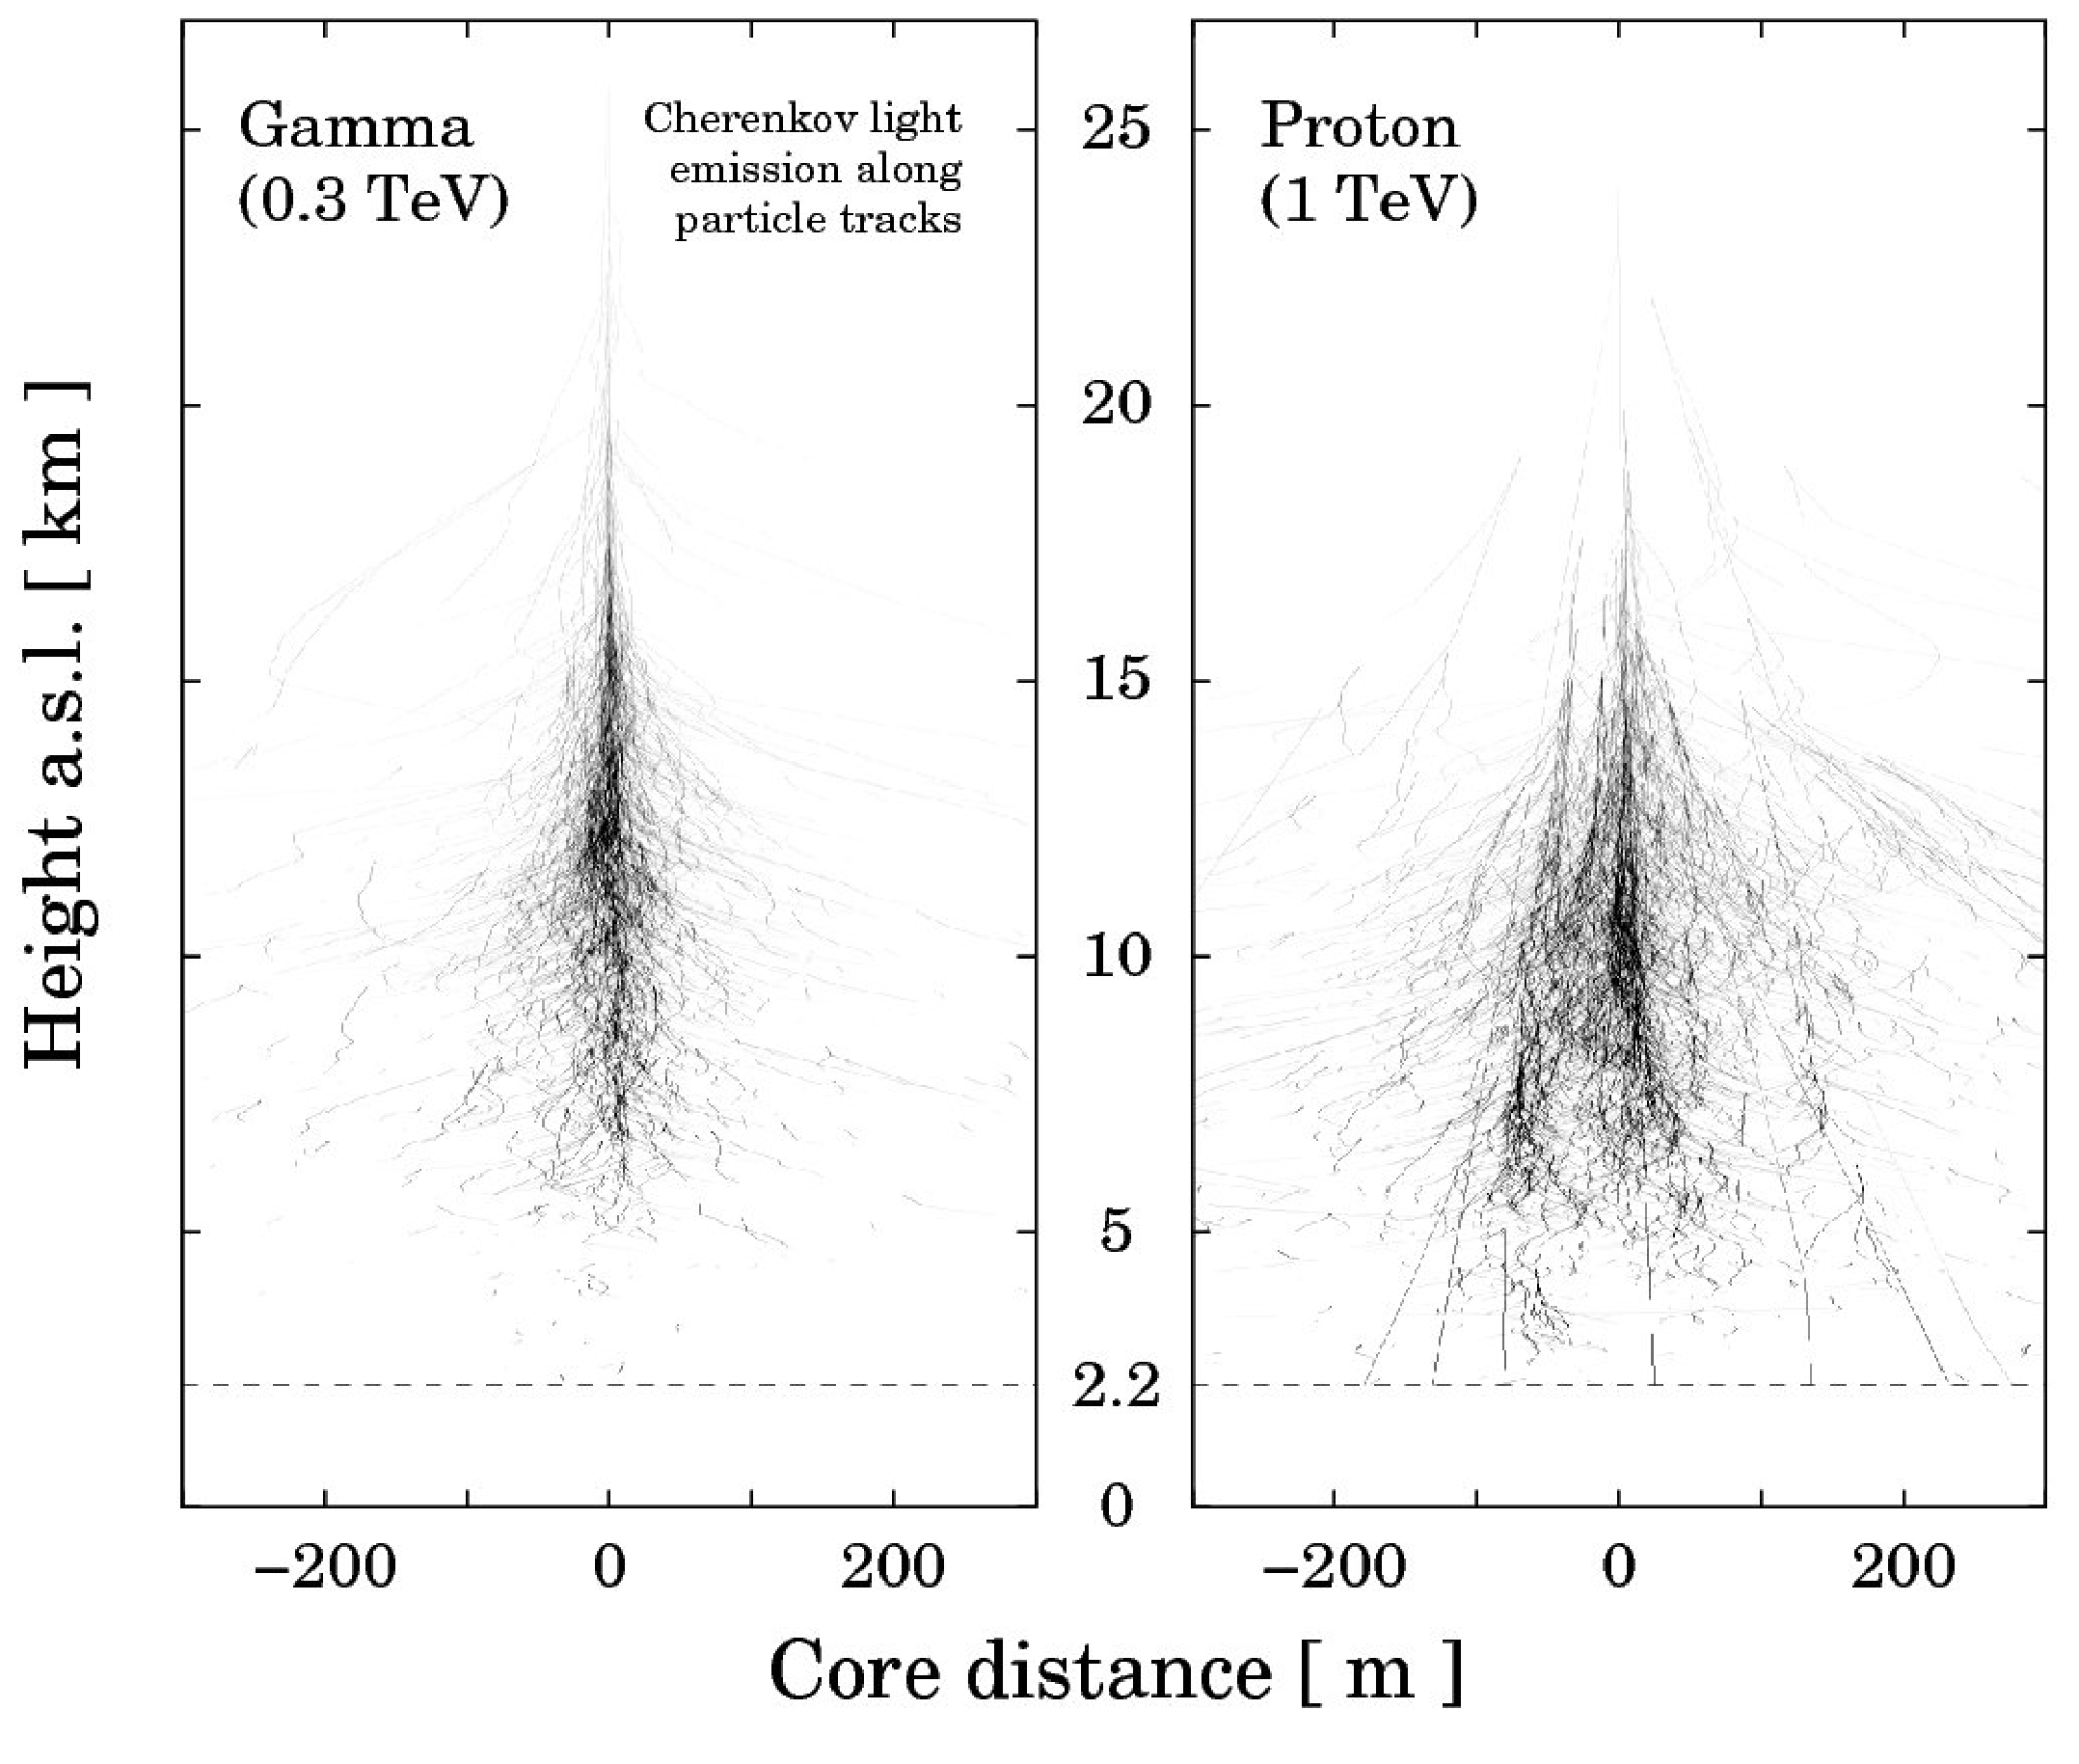
\includegraphics[width=0.95\textwidth]{images/showers_gamma_proton}
    \caption[Gamma Ray and Proton Showers]{
      A gamma ray shower alongside a proton shower~\cite{Bernlohr2008149}.
    }
    \label{fig:gamma_vs_proton_airshower}
  \end{figure}
  
  \FloatBarrier

  \subsection{Cherenkov Photons}\label{sec:cherenkov}

  Within atmospheric showers, any charged particles travelling at velocity $v > c_{atmosphere}$, where $c_{atmosphere}$ is the speed of light in the atmosphere, will induce the atmosphere to produce Cherenkov photons~\cite{cherenkov}.
  From a single charged particle of constant velocity, Cherenkov photons form a conical wavefront shown in Figure~\ref{fig:cherenkovangle}, similar to a sonic boom shockwave or the wake produced when a boat travels faster than the speed of the waves.

  \begin{figure}[ht]
    \centering
    \includegraphics[width=0.27\textwidth]{images/cherenkov_angle/cherenkovangle.pdf}
    \caption[Chernekov Emission Angle]{
      Cherenkov light (blue arrows) is emitted at angle $\theta$, relative to the charged particle z's path.
    }
    \label{fig:cherenkovangle}
  \end{figure}

  Cherenkov photons are produced at an angle $\theta$ relative to the charged particle's path, determined by the index of refraction of the medium $n$, the speed of the charged particle $v$, and the speed of light in the medium $c$, as in Equation~\ref{eqn:cherenkovangle}.

  \begin{equation}\label{eqn:cherenkovangle}
    \theta = ArcCos \left ( \frac{c}{n \; v} \right )
  \end{equation}
  
  For the gamma-ray showers used in this analysis, the cherenkov angle $\theta$ is \nicetilde\ang{1}.
  {\color{red}(Is it only for the gamma-ray showers this angle?? -orel)}
  % showers are 10km up, light pool on ground is 130m diameter, \theta = ArcSin(130/10000) * 180 / pi = 0.73deg ~ 1deg

  However in an atmospheric shower, the number and distribution of charged particles and their velocities, as well as energy losses, tend to smear the theoretically-clean Cherenkov cones into a diffuse pool of light on the ground, shown in Figure~\ref{fig:lightpool}.

  \begin{figure}[ht]
    \centering
    \includegraphics[width=0.85\textwidth]{images/lightpool/lightpool.pdf}
    \caption[Chernekov Light Pool]{
      Cherenkov light from a gamma ray shower illuminating the ground.
      Due to the changing atmospheric density, the cherenkov angle changes as the electromagnetic shower decends (Left), concentrating the emitted light into a ring-like pool (Right).
      The initial gamma ray had an energy of \SI{1}{\TeV}.
      Figure is from Ref.~\cite{Voelk}.
    }
    \label{fig:lightpool}
  \end{figure}
  
  The spectrum of photons produced by the Cherenkov effect can be calculated with the Frank-Tamm formula~\cite{franktamm1,franktamm2} in Equation~\ref{eqn:franktamm},
  
  \begin{equation}\label{eqn:franktamm}
    \frac{dE}{dx\,d\omega}=\frac{(ze)^2 \, \omega}{c^2} \left ( 1 - \frac{c^2}{v^2 \;\epsilon(\omega)} \right )
  \end{equation}
  
  where $E$ is the energy emitted as Cherenkov radiation, $x$ is the length of the charged particle path, $ze$ is the charge of the particle, $\omega$ is the emitted Cherenkov photon frequency, $c$ is the speed of light (phase velocity) in the medium, $v$ is the speed of the particle, and $\epsilon(\omega)$ is the frequency-dependent permittivity.
  The UV- and visible-spectrum Cherenkov photons are then imaged and recorded by the VERITAS observatory.
  
  \begin{figure}[ht]
    \centering
    \includegraphics[width=0.75\textwidth]{images/CherenkovReactor/cherenkovreactor.eps}
    \caption[Chernekov Light from a Reactor]{
      Blue Cherenkov light in the Advanced Test Rector core, at the Idaho National Laboratory~\cite{cherenkovreactor,atrlab}.
    }
    \label{fig:cherenkovreactor}
  \end{figure}
  
  In Figure~\ref{fig:cherenkovreactor}, a visible example of Cherenkov photons is shown, produced in the Advanced Test Reactor at the Idaho National Laboratory.
  Neutrons emitted by the reactor collide with atoms in the water, freeing some electrons with enough kinetic energy to travel faster than the speed of light in water.
  These superluminal-in-water electrons then create the blue Cherenkov photons imaged here.
  

\cleartooddpage[\thispagestyle{empty}]
\chapter{Veritas}

\section{Observatory}
Look at this observatory, its so awesome!

\section{Hardware}

\section{Effective Area}

\section{Energy Resolution}

\section{Point Spread Function}

\section{Energy Sensitivity and Zenith Angle}

\section{Comparison with Other Observatories}
HAWC, Fermi

\cleartooddpage[\thispagestyle{empty}]
\chapter{Gamma Ray Reconstruction}\label{ch:grrecon}

In chapter \ref{chapter:veritas}, it was explained how the trigger system preserves PMT voltage traces of potential events.
To reconstruct gamma rays, the voltage traces caused by cherenkov photons must be identified and combined to form an image of the original cherenkov shower.
Then the shower images from multiple telescopes can be used to reconstruct the original gamma ray's energy and direction.

\section{Pedestal Variation}
Before reconstructing any events, the pedestal and pedestal variations must be calculated.
These are done by artificially triggering all pixels once per second during normal data-taking, in order to record events that solely contain noise.
The average of the digital counts (dc) of all noise-events for each pixel is then the pedestal.
From this pedestal, the pedvar is then calculated as the rms of the all the dc counts in all noise-events, which can be visualized as the distribution of dc around the mean dc.

(also see \cite{Hanna2010NIM} about relative gains??)

\section{Pixel Identification}
The first step is to determine which pixels are part of a shower image or not.
This is done by subtracting the digital counts pedestal from the entire trace, and then integrating the total dc in each voltage trace.
In addition, the time when the voltage trace is at half of its maximum value, called $T_{0}$.

Around time $T_{0}$, the trace is integrated a second time with a smaller time window (usually either 14 or 24 ns wide, 30\% of the window before $T_0$), to reduce the inclusion of dc from sources of noise (NSB and electronics).
This two-pass algorithm is usually referred to as the double-pass method (cite??).
If a pixel's second-pass total dc is higher than 5 times the pedvar, then it is considered an image pixel.
If it is between 2.5 and 5 times the pedvar, it is considered a border pixel.

Once all pixels have been classified, isolated border pixels that have no neighboring image pixel are also removed, as they are more likely to be due to noise than cherenkov photons.
Then, the time gradient from the image and border pixels can be found by examining a linear fit of the $T_{0}$ times.
This gradient can then be used to place a third integration integration window with 30\% of the window before each pixel's $T_{0}$, to more accurately measure the charge due to cherenkov photons in the pixel.

From the image pixels, border pixels, and time gradient, the shower's Hillas parameters can be calculated.
These include the size of the shower in photoelectrons (or equivalent units), the shower center of charge, angle, length and width.
The center of charge is the charge-weighted average of all image and border pixel positions.
The angle of the shower determines how the image's major axis is oriented in the camera.
The shower length and width are determined by the rms of the shower image along its major and minor axes, respectively.


\section{Position Reconstruction}\label{subsec:posrecon}
By examining the images from multiple telescopes, the initial position of the event can be determined.
This is done by overlapping all telescope images in a single camera coordinate system, and projecting each image's major axis backwards in time.
These drawn lines should intersect very close together, and a weighted average of the intersection points determines the event's initial direction.

In averaging the intersection points, weighting for each intersection can be applied based on the angle between the two lines.
This improves the reconstruction, because the intersection point from two images at 90\degree angles will be less sensitive to image fluctuations than two images at 160\degree, as shown in figure \ref{fig:largeintersectangle}.
Additionally, the disp method can be utilized to offer improvements in the lower elevations.

\begin{figure}[ht]
  \begin{center}
    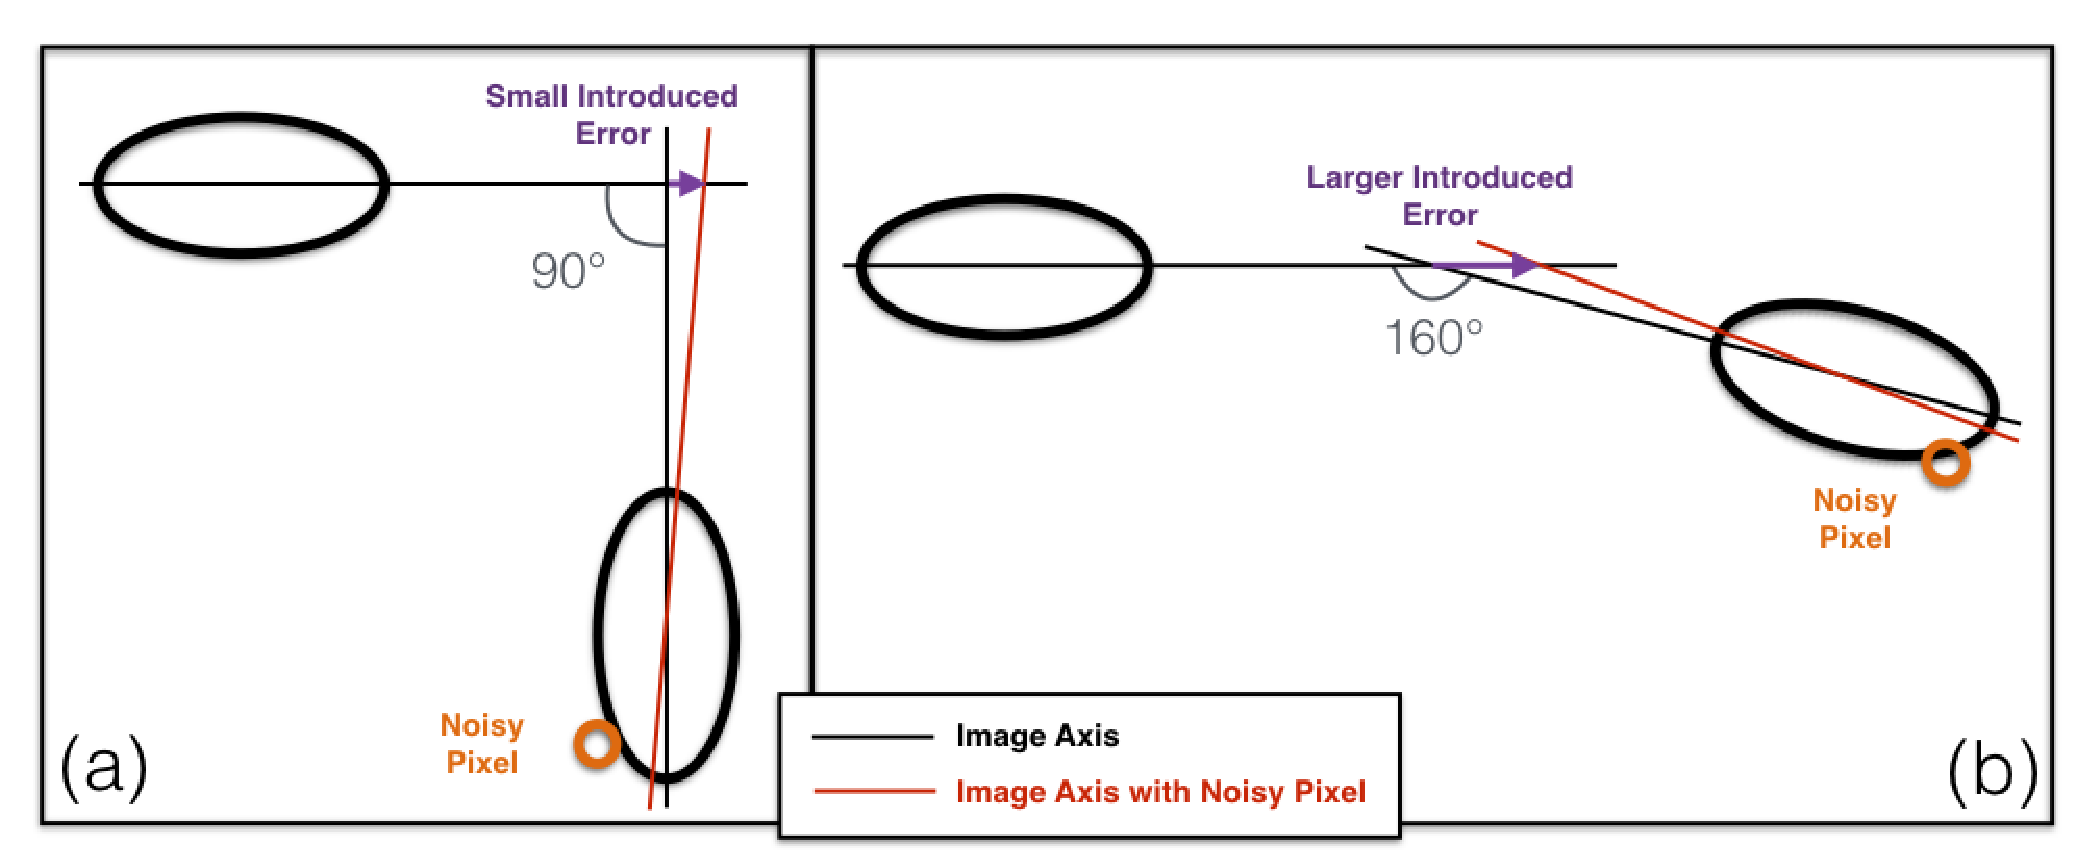
\includegraphics[width=0.95\textwidth]{images/large_angle_image_intersection_error_cropped.eps}
    \caption[Large Image Intersection Angles]{In diagram (a), when a noisy pixel is added to an image, the reconstructed position is only moved a small distance (the purple arrow).  In diagram (b), due to the large angle between images, the reconstructed position is much larger.}\label{fig:largeintersectangle}
  \end{center}
\end{figure}

\subsection{Angular Reconstruction Neural Network}\label{subsec:disp}
At high elevations, shower images are often at large intesection angles, because the telescopes are spread out in two dimensions, relative to the shower in the atmosphere.
At low elevations near the galactic center, however, the telescope array flattens into one dimension, which makes the shower's impact parameter (the shortest distance between the telescope and the shower core axis) smaller for two of the telescopes.
These two closer telescopes then have very short, almost circular images, which increases the sensitivity of those two image axes to noisy pixels or shower fluctuations, as shown in figure \ref{fig:showerhighlowelev}.
This also causes the remaining telescope images to have large intersection angles, which also reduces the accuracy of the position reconstruction.

\begin{figure}[ht]
  \begin{center}
    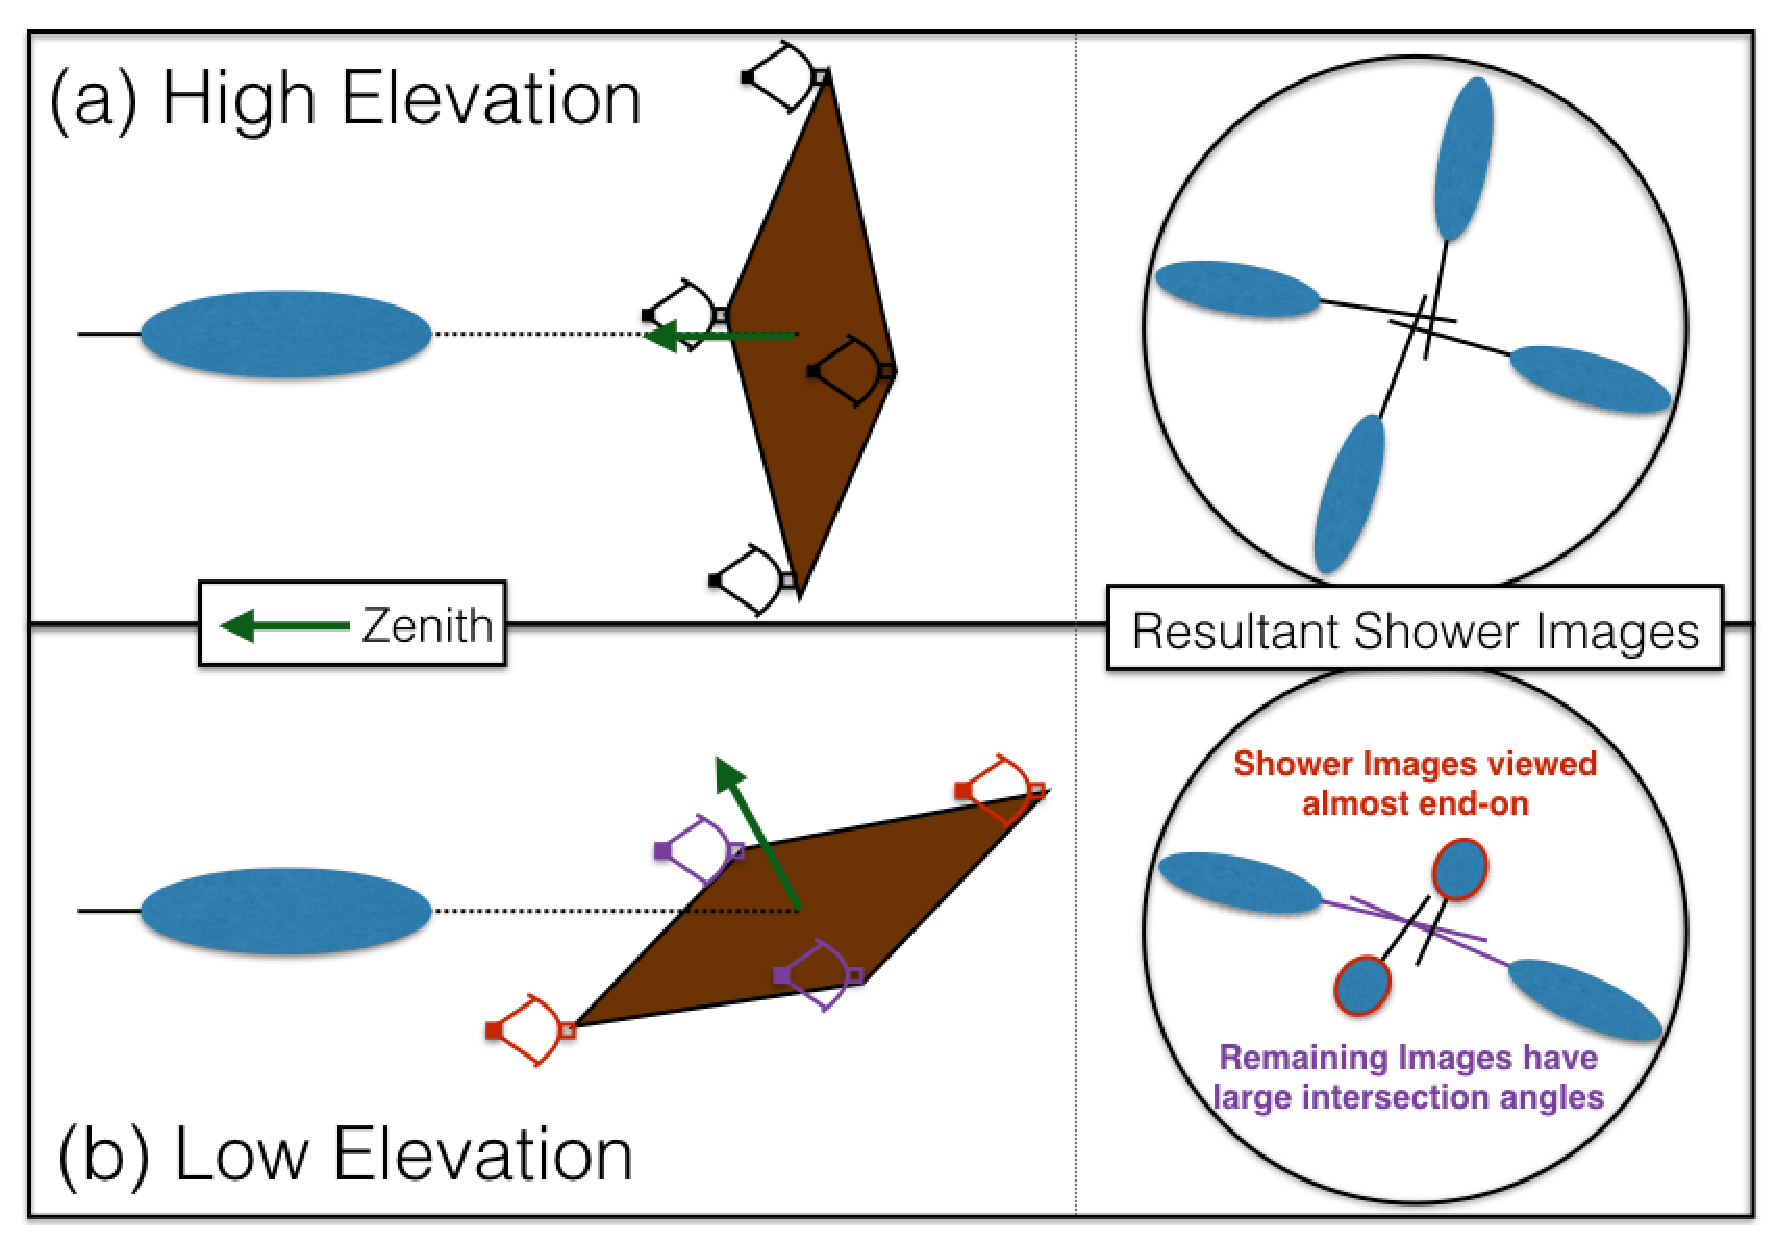
\includegraphics[width=0.75\textwidth]{images/high_elevation_vs_low_shower_images_cropped.eps}
    \caption[Shower Images at High and Low Elevations]{In figure (a), high elevation showers produce long images in all four telescopes.  In figure (b), lower elevation showers produce shortened images in two telescopes, and the remaining images form large angle intersection.}\label{fig:showerhighlowelev}
  \end{center}
\end{figure}


To better handle these near-parallel image axes at low elevations, the reconstructed position can be determined from more parameters than just the weighted image axes intersection points.
From simulations, the distance between the center of the hillas shower image and the reconstructed position can be calculated, where the angular distance between the two is the 'disp' parameter\cite{Senturk:2011}, shown in figure \ref{fig:dispdiagram}.
Then, a machine learning algorithm \cite{Beilicke2012NIM} can be trained on these simulations at various energies and positions in the camera(??).
This algorithm's disp-predicted positions can then be weighted and included in the intersection averaging.

\begin{figure}[ht]
  \begin{center}
    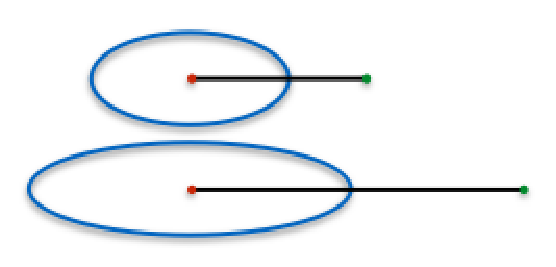
\includegraphics[width=0.5\textwidth]{images/disp_parameter_cropped.eps}
    \caption[Angular Reconstruction Disp]{The disp parameter is the angular distance between the center (red dot) of a hillas image (blue oval) and the true sky position (green dot).  Generally, longer shower images have a larger disp angle.}\label{fig:dispdiagram}
  \end{center}
\end{figure}

% https://veritas.sao.arizona.edu/wiki/index.php/BDT_Angular_reconstruction
The disp and other parameters for thousands of simulated showers can then be used to train a boosted decision tree forest (BDT) that estimates the most probable disp for a given shower.
This most probable disp can then be used with the image axes intersection points to more accurately reconstruct the original gamma-ray point of origin.

Once the training is complete, it is tested on a separate set of 17,000 simulated events, which are plotted in figure \ref{fig:disptraining}.
The x axis describes the true disp value for each event, while the y axis describes the disp value estimated by the BDT, with a black line for the x=y line, which represents a perfect disp reconstruction.
As the majority of the events fall on the line, it can be concluded that the BDTs are able to predict the correct disp value for most images.

% made from screenshot of last slide in Dropbox/Presentations/20160719_Group_Meeting.key
\begin{figure}[ht]
  \begin{center}
    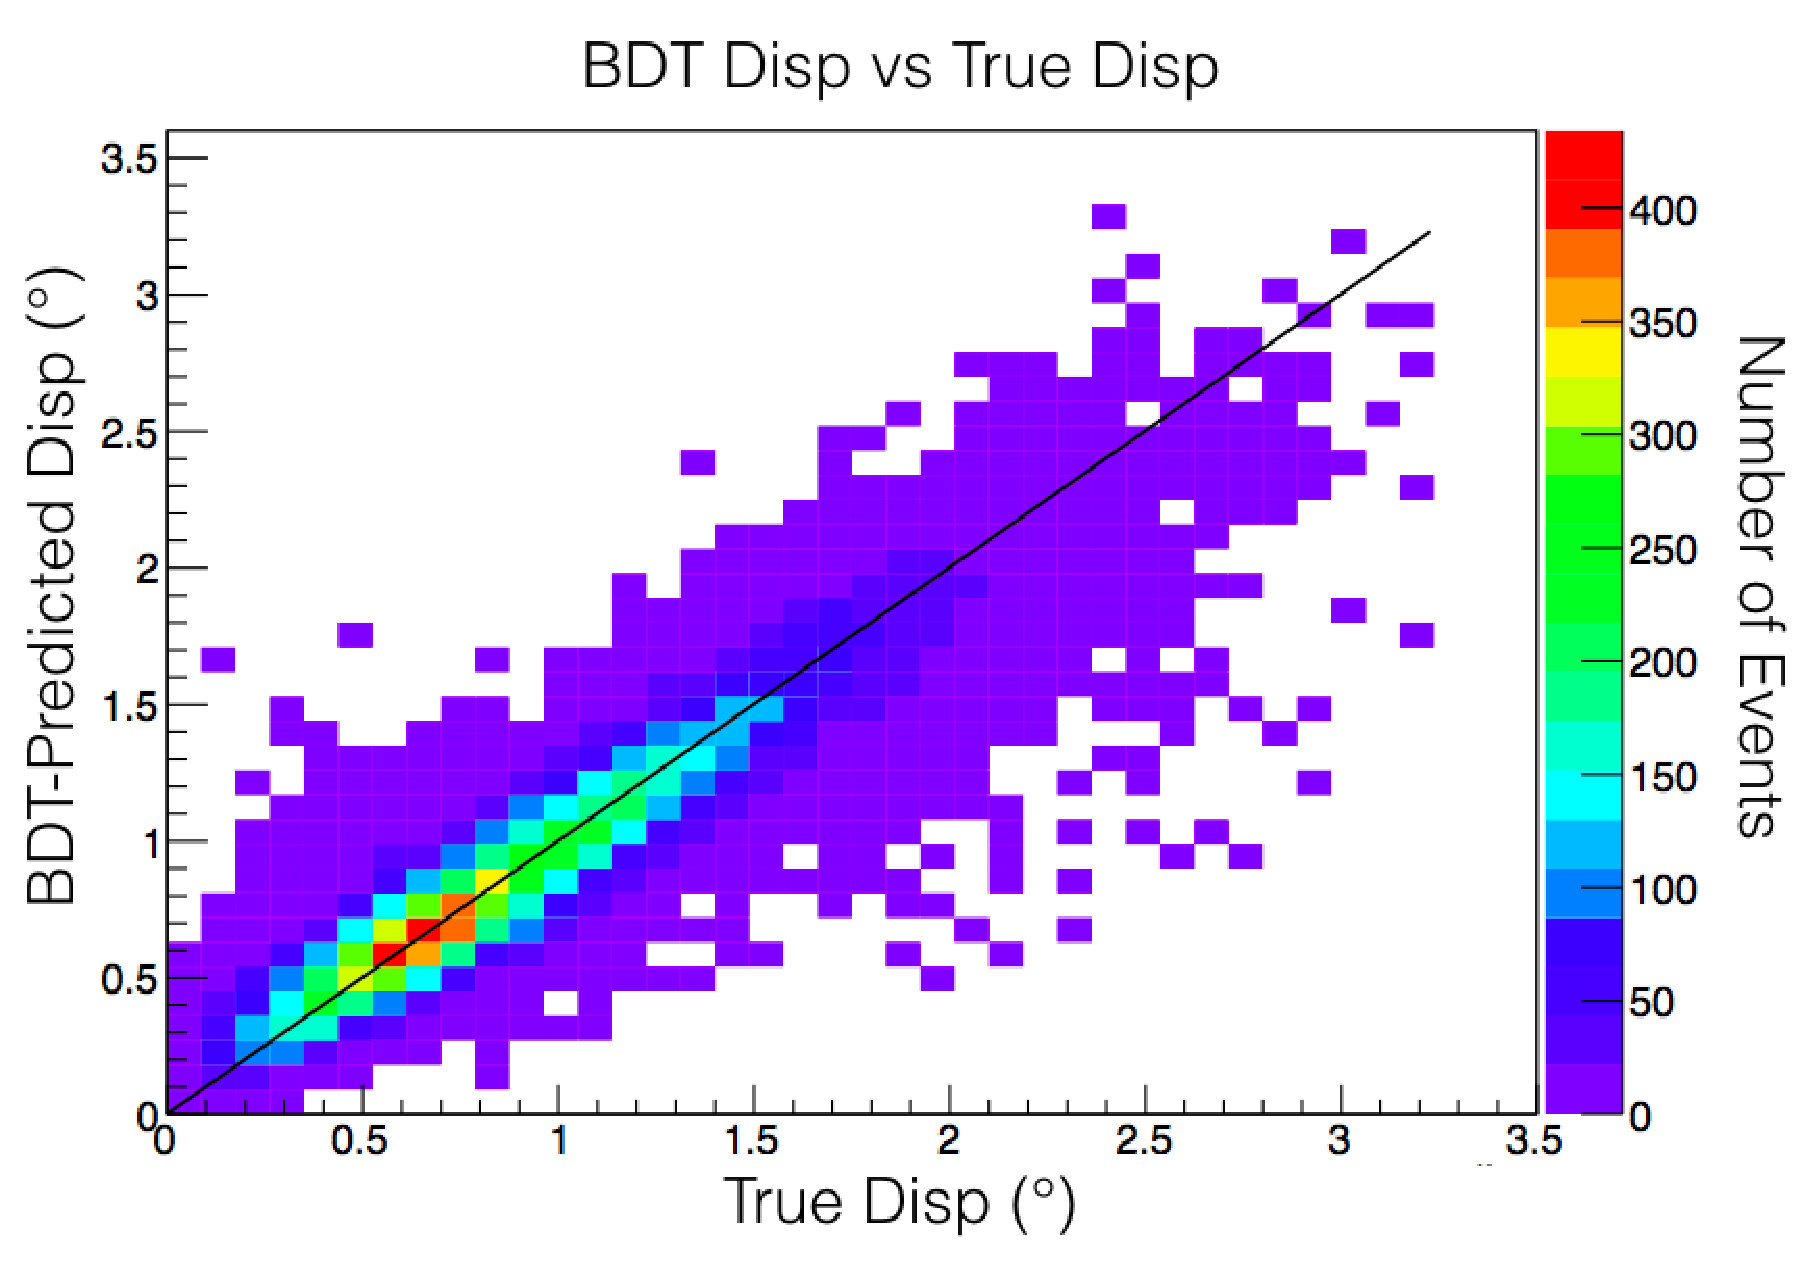
\includegraphics[width=0.85\textwidth]{images/disp_training.eps}
    \caption[Disp BDT Training]{The true disp vs the BDT-predicted disp, for \nicetilde17,000 gamma-ray event images in T1, from 500GeV to 200TeV.}\label{fig:disptraining}
  \end{center}
\end{figure}

The small improvement in the position reconstruction due to the disp method can be seen in figure \ref{fig:disp_event_offset}.
With the Geometric (red) events, more are concentrated further from the point source, while with the Disp method, somewhat more are concentrated at the source itself.

\begin{figure}[ht]
  \begin{center}
    \includegraphics[width=\textwidth]{images/disp_event_offset_hists/disp_event_offset_hist.eps}
    \caption[DISP Offset Improvement]{The number of events at different angular offsets from the Crab and the Galactic Center, with both Geometric and Disp reconstruction methods.}\label{fig:disp_event_offset}
  \end{center}
\end{figure}


\section{Energy Reconstruction}\label{subsec:enrecon}
To reconstruct the energy of each shower, a database of simulated showers is built.
This database includes the width and length of the shower, how far away its core position is, how bright it was, as well as its reconstructed and true energy.
By scanning through this database for showers that are similar to the one being constructed, the most similar-looking shower then indicates the true energy(??).



\section{FITS Conversion for Gammalib and CTOOLs}

Once gamma rays have been reconstructed with event display, they must be converted to a FITS file format compatible with Gammalib and Ctools.
This format consists of a FITS file with an event list table, containing each gamma ray, its energy, sky direction, and time.
This also includes meta information about the event list like the telescope's pointing target and the start and end times of the event list.
This FITS file can then be read into Gammalib and CTOOLS \cite{gammalibctools}.

In addition to the event list, the instrument response functions (IRFs) must also be imported into Gammalib and Ctools.
These include effective areas, point spread functions, energy dispersion, and background models for several dimensions in the IRF parameter space (energy, offset from camera center, telescope elevation/azimuth, NSB noise, etc).
By default, all IRFs are stored in a single database, and each event list contains a reference to which part of the parameter space should be used with it.

However, the galactic center is at an elevation of $\ang{30}$, much lower than most VERITAS observation targets.
At this elevation, with its field of view of $\ang{3.5}$, the air mass column density ($g/cm^{2}$) is 20\% higher at the bottom of the camera than at the top.
Add to this that during a single 30 minute observation, the elevation of the Galactic Center can change by several degrees, means the airmass in view of the camera may change rapidly, meaning the IRFs may become time dependent.

To allow for the inclusion of this time dependence in the analysis, an alternate way of storing the IRFs was chosen, diagrammed in figure \ref{fig:fits_scheme}.
First, one observation (typically 20-30 minutes long) is broken up into \nicetilde8 minute chunks.
Each chunk is then converted to an event list, and saved to a FITS file.
In addition, the needed Effective Area, PSF, and background models are also written to the same FITS file.
As each event list covers a small region in time, the IRF tables only need to contain the dimensions of the parameter space that can change during one chunk, such as event energy and distance from camera center.

\begin{figure}[ht]
  \begin{center}
    \includegraphics[width=0.75\textwidth]{images/FITS_diagrams_alternate_scheme.eps}
    \caption[FITS File Event Storage Schemes]{}\label{fig:fits_scheme}
  \end{center}
\end{figure}

The end result is that a 30 minute observation can be broken into several FITS files (called chunks), where each chunk file is independent of any outside references, contains all needed IRF information, and only takes up \nicetilde100s KB on disk.
This makes it ideal for an analysis program to automatically download any needed data over an internet connection, as each chunk is tiny and has no outside dependencies.
As gammalib and CTOOLS expect the default FITS file scheme, a python function was written to automatically load all event and irf tables from a single fits file, and import this information into gammalib's GObservation class.

There were minor issues with converting the IRFs that are noted in the following sections.

\subsection{Effective Area}\label{sec:effarea}
% plot of effective area vs energy
Effective area is the measure of how large an observatory's collection area is, determining how many gamma rays are be detected per unit time, solid angle, and energy.

For each point in the parameter space, the effective areas are calculated with many Monte Carlo gamma ray simulations.
This is done in the shower plane, the plane perpendicular to the line drawn between an observing source, and the center of the observatory.
The effective area is then calculated via:
$A=\pi R^2 \frac{N_{survived}}{N_{simulated}}$
where R is the radius of the area within which simulated showers are directed to fall, $N_{simulated}$ is the number of showers that were initially simulated into the area, and $N_{survived}$ is the number of simulated showers that pass all cuts.
This 'Effective' area is thus a measure of how much detection area the observatory would have if it had a 100\% detection efficiency, which can then be used in calculating a source's flux.

\begin{figure}[ht]
  \begin{center}
    \includegraphics[width=0.75\textwidth]{images/effarea_plots/effarea_parameter_space.eps}
    \caption[Effective Area Parameter Space]{Effective areas at different points in the Energy and Camera Offset parameter space for run 78128.}\label{fig:effarea_paramspace}
  \end{center}
\end{figure}

For the test analyses of the Crab and the Galactic Center Point Source, the effective areas of all events are shown in figure \ref{fig:effarea_usage}.

\begin{figure}[ht]
  \begin{center}
    \includegraphics[width=\textwidth]{images/effarea_plots/effarea_usage.eps}
    \caption[Effective Area Parameter Space]{Effective Areas used by events in each analysis.}\label{fig:effarea_usage}
  \end{center}
\end{figure}

\subsection{Point Spread Function}\label{sec:psf}

In addition to the energy being slightly mis-reconstructed, the source position of the gamma ray can also be misreconstructed.
For VERITAS, this misreconstructions are measured by simulating many gamma rays in the camera, and looking at the distribution of true positions for a given reconstructed position, which is called the point spread function (PSF).
To first order, most current-generation point spread functions are gaussian distributions.
For Event Display, the PSF has been roughly measured to be gaussian-shaped.
For CTOOLS instead, a King function (Eqn \ref{eqn:king}) was fitted to the distribution of events, as Fermi and HESS have found (cite??) gamma ray PSFs tend to have longer tails than a Gaussian, which the king function better handles.

The psf is the distribution of true event directions for a given reconstructed event direction.
Within an analysis, the event PSF strongly depends on the event energy, as well as its distance from the camera center.

In order to use Event Display's psf in ctools, some conversion is necessary.
Event display natively stores its psf as a pair of 68\% and 80\% containment radii (referred to as $r_68$ and $r_80$, respectivly), each as a distance in degrees between the monte carlo event direction and the reconstructed direction.
These radii contain 68\% and 80\% of all events in the distribution, and are used to fit a gaussian profile.
For ctools, a king function is used instead of a gaussian.

\begin{equation} \label{eqn:king}
$$ psf_{king}(r) = \frac{1}{2 \pi \sigma^{2} } \left( 1 - \frac{1}{\gamma} \right) \left( 1 + \frac{ r^{2} }{ 2 \gamma \sigma^{2} } \right)^{-\gamma} $$
\end{equation}

where $r$ is the angular distance from the reconstructed position, $\sigma$ is similar to the width of a gaussian , and the $\gamma$ parameter affects how long the tails are.
The function is integrates to 1 in polar coordinates with $r$ in radians.

A king function fitting algorithm was added, that fits for the $\gamma$ and $\sigma$ parameters, from the same distribution of events that the r68 and r80 radii are calculated from.
This leads to good fits over almost all of the parameter space.

(example fit image of distribution of events and fitted king function ??)

A smaller psf is important for this analysis, as the presence of a dark matter halo relys on the pointing accuracy of the events around the galactic center.
A worse gamma-ray psf (with a wider distribution of possible true positions) will smear out any dark matter halo around the galactic center, making its detection more difficult.

In figure \ref{fig:psf_paramspace}, the psf is shown for one Galactic Center run.
In it, one can see how the psf containment radius changes vs reconstructed energy and offset from the camera's center.
Other runs, which have different elevations, azimuths and NSB noise levels will have different values at each point in the energy/offset parameter space.

% plot of psfs from chunkplot
\begin{figure}[ht]
  \begin{center}
    \includegraphics[width=0.75\textwidth]{images/psf_king_plots/psf_parameter_space.eps}
    \caption[PSF Parameter Space]{The 68\% containment radius for the Energy/Offset parameter space for Galactic Center run 78128.}\label{fig:psf_paramspace}
  \end{center}
\end{figure}

For the Galactic Center analysis, the 68\% containment radius for all events was histogrammed into figure \ref{fig:gc_psf_hist}.

\begin{figure}[ht]
  \begin{center}
    \includegraphics[width=\textwidth]{images/psf_gc_eventhist/eventpsfhist.eps}
    \caption[Crab and Galactic Center Event PSFs]{The 68\% containment radius for all Galactic Center and Crab events used in this analysis.}\label{fig:psf_paramspace}
  \end{center}
\end{figure}

\subsection{Background Templates}

To produce a background, events are binned in camera coordinates and energy.
The energy bins are determined by expanding outwards (in $log_{10}(TeV)$ space) from the median energy of all events, until each energy bin has at least 100 events per degree$^2$, expanding to include any energy ranges that have less than that.
In these energy bins, events are then binned radially, which is then used to fit an interpolation function (see figure \ref{fig:background_radial}), which is then normalized to one when integrated around the entire camera, which is the pdf of one event.
These energy-bin pdfs can then be interpolated linearly in $log_{10}(TeV)$ space, to get the radial distribution of events at various energies.

\begin{figure}[ht]
  \begin{center}
    \includegraphics[width=\textwidth]{images/ctools_background/radial_profiles.eps}
    \caption[CTOOLS Radial Background Profiles]{Radial bin profiles for the V5 background's two large-scale energy bins.  (These plots need axes labels, and the blue error bars are not accounting for the bin area properly!??).  The blue points are the counts per bin area, while the purple line is the interpolation with a spline interpolator of order 3 (see scipy.interpolate.interp1d())}\label{fig:background_radial}
  \end{center}
\end{figure}


Then, all events are divided up into \nicetilde30 finer energy bins as shown in figure \ref{fig:background_profile}, and each bin's counts are multiplied by the interpolated radial pdf at that energy, which is then written to a two-dimensional array of camera x/y bins.
2D bin values are then divided by the solid angle of the bin (in sr), the energy width of the bin (in Mev), and the total obseration time (in seconds).

\begin{figure}[ht]
  \begin{center}
    \includegraphics[width=0.9\textwidth]{images/ctools_background/background_construction.eps}
    \caption[CTOOLS Background Fine Energy Bins]{The V5 Background's fine-energy bins.  The left plot shows the number of events in each fine-energy bin.  The right plot shows the ctools background values.  The black lines show the fits background value and energy bin width saved to the background file, while the blue line shows the background value after ctools loads and interpolates those fits background values.  Note the y-axis in the left plot is linear, while in the right plot, it is $log_{10}$. (These plots should be cleaned up a little??)}\label{fig:background_profile}
  \end{center}
\end{figure}

Additionally, three extra 'zero' background maps (with an extremely low value of $10^-13 \frac{counts}{Mev s sr}$ are added above and below the fine energy bins, so that the ctools background interpolation will properly predict the correct lack of events above and below the energy range.

The background is used in the likelihood analysis as a model with one free parameter, a simple multiplicative normalization factor.
This lets the likelihood engine scale each run's background model up or down to best fit the events, so the background's absolute value is less important than the relative values in different parts of the camera.
Indeed, it was noticed that during background fitting, the normalization factor was usually around $\frac{1}{150}$, so future backgrounds were created with this value multiplied in already, which reduced the likelihood runtime from around 7-9 hours to 2 hours for the galactic center point source analysis.
The background normalization factors after the $\frac{1}{150}$ adjustment were shown to be centered around 1.0, varying from from 0.5 to 1.5.


\subsection{Energy Dispersion}
As events are reconstructed imperfectly, it can be important to understand what the distribution of true energies are for a given reconstructed energy.
In an analysis with ctools, this is quantified by an energy dispersion matrix, that indicates the number of simulated events at each $(E_{reconstructed},E_{true})$ point in a matrix.
As the likelihood engine in ctools did not at the time of this analyis have energy dispersion fully incorporated, it was not used in this analyis.
This is accounted for by adding ??\% to the total systematic error.



\section{New Background Behavior}

During the production of the initial low elevation backgrounds, some new effects were noted.
First, a series of gamma-like events were taken from observations with no known gamma-ray sources.
These events were then divided into equal-statistics energy bins.
For each equal-statistic energy bin, all the contained events are binned in camera X and Y.

For a set of high-elevation observations, these backgrounds are shown in figure \ref{fig:back_highelev}.
It can be seen that all events are divided up into 3 equal-statistics energy bins in figure \ref{fig:back_highelev}.A.
Each energy bin is then binned in camera X and Y in figure \ref{fig:back_highelev}.B, .C, and .D.
It can be seen that at these high elevations, each energy bin is radially symmetric about the camera center.
This happens because gamma ray's point of origin and its shower image in the camera are usually several tenths of a degree away from each other.

\begin{figure}[ht]
  \begin{center}
    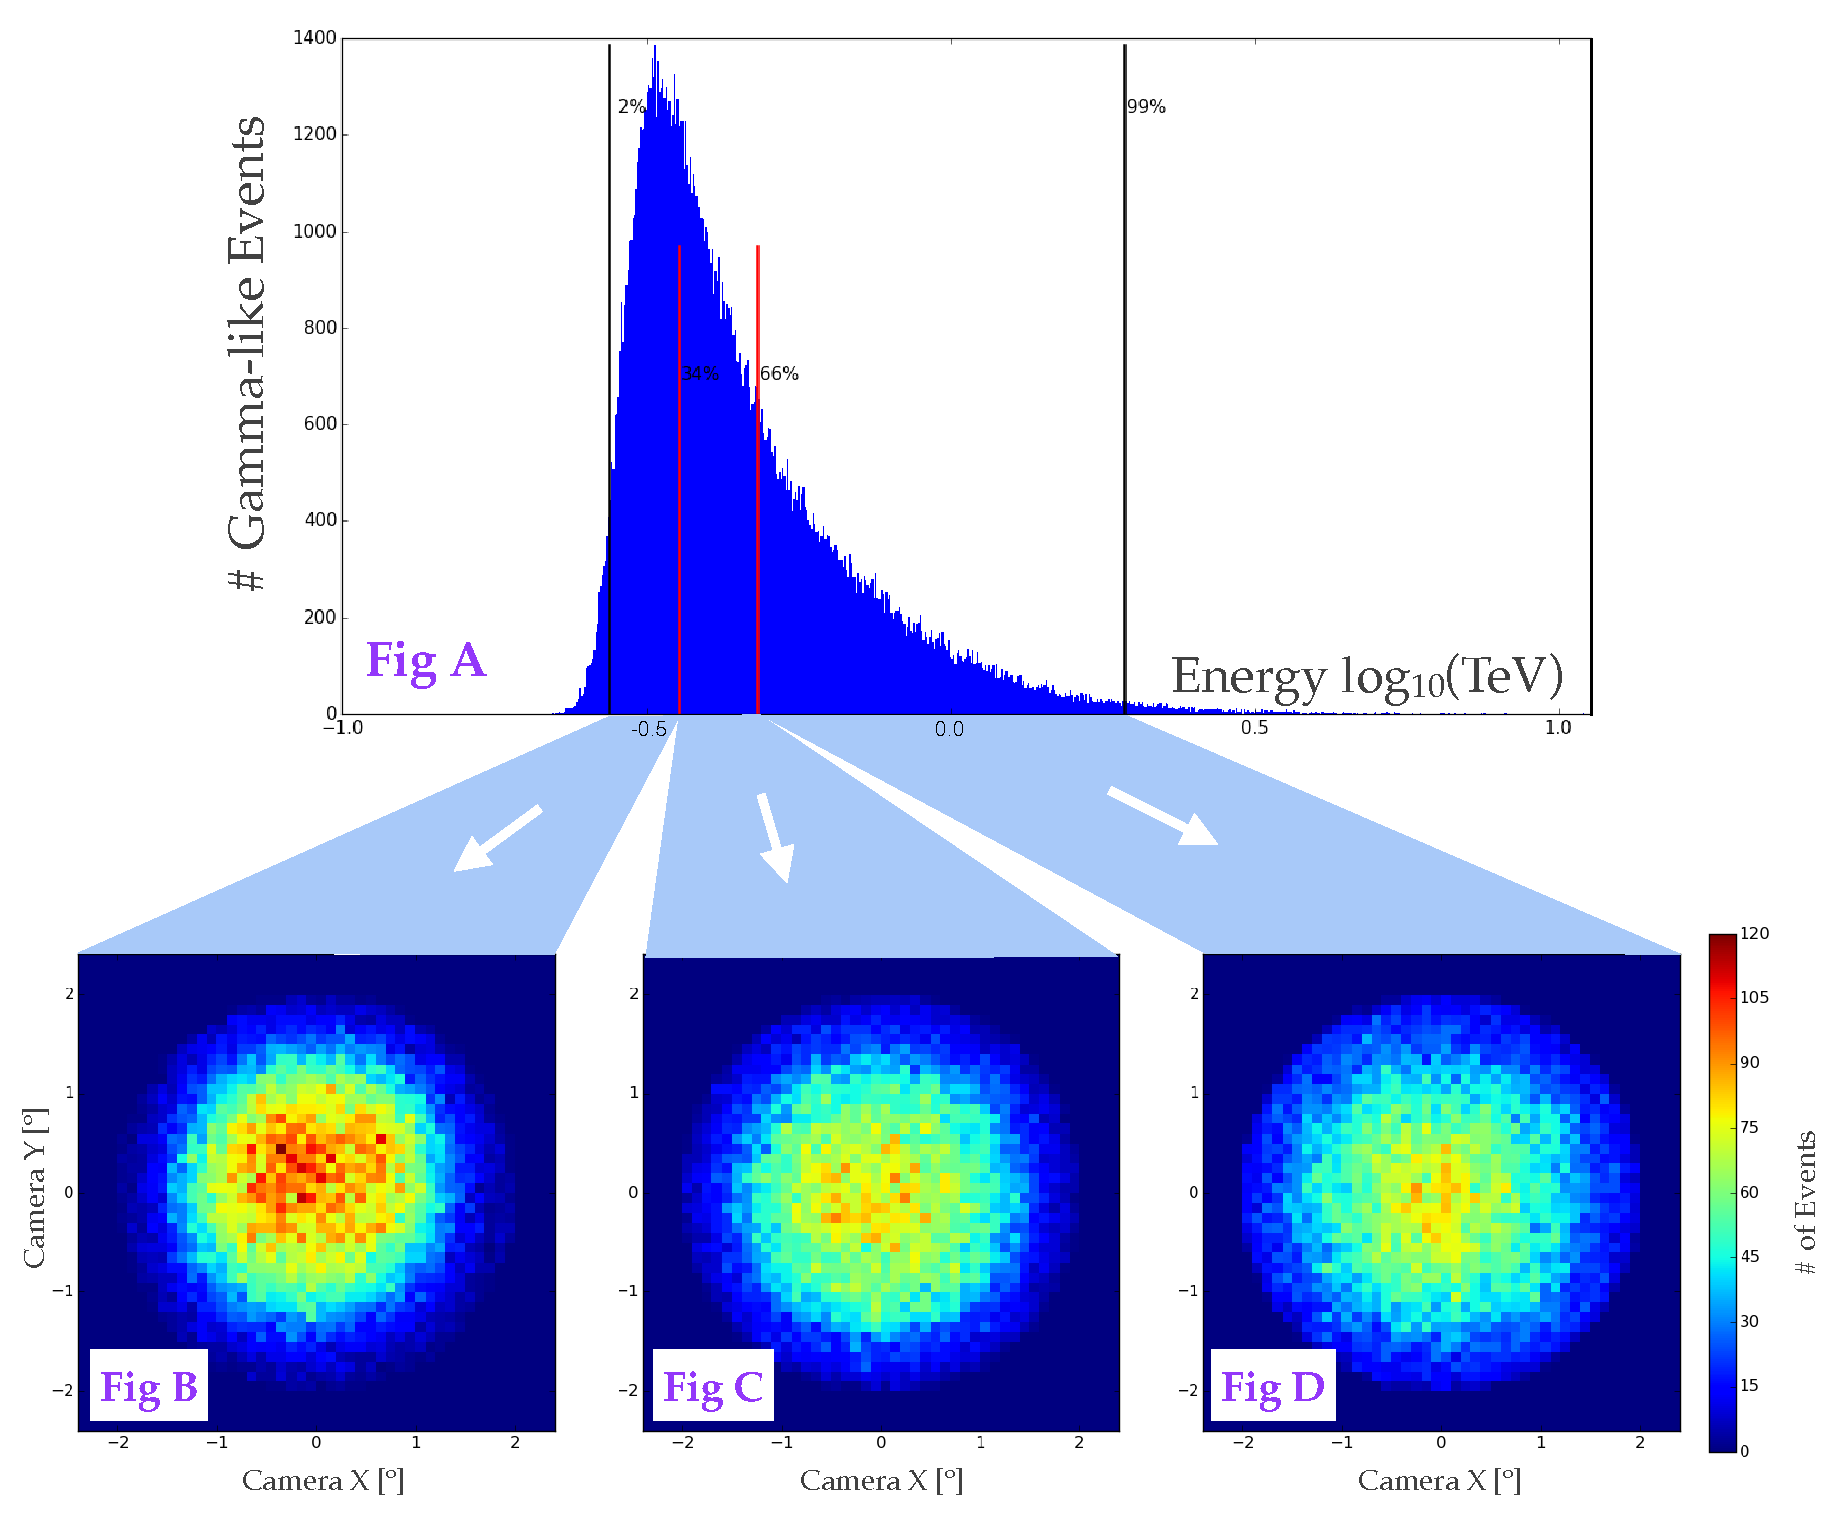
\includegraphics[width=\textwidth]{images/ctools/backgrounds_highelev.eps}
    \caption[FITS Background at 50\degree Elevation]{Gamma-like Events from 52 observations (approximately \nicetilde20 hours) of M82, between 50\degree  and 52\degree  elevations.  Events in Figure A are divided into 3 equal-statistics energy bins, and binned in Camera Coordinates in Figures B, C, and D.}\label{fig:back_highelev}
  \end{center}
\end{figure}

In figure \ref{fig:back_lowelev29} and figure \ref{fig:back_lowelev26}, the same plots are constructed for a set of low-elevation ($ \nicetilde \ang{29} $ and $ \nicetilde \ang{26} $ respectivly)) observations, using Galactic Center Off observations.
These are again divided in to equal-statistic energy bins, and then each energy bin is binned in camera coordinates.
It can be seen that in different energy bins, the background possesses different shapes.

\begin{figure}[ht]
  \begin{center}
    \includegraphics[width=\textwidth]{images/ctools/backgrounds_lowelev29.eps}
    \caption[CTOOLS Background at 29\degree Elevation]{15 Sagittarius A* Off runs (\nicetilde7.5 observation hours), between elevations $ \ang{27.5} $ and $ \ang{30} $.  Events are divided into 6 equal-statistics energy bins, of which four are binned in Camera Coordinates in figures B, C, D, and E.}\label{fig:back_lowelev29}
  \end{center}
\end{figure}

\begin{figure}[ht]
  \begin{center}
    \includegraphics[width=\textwidth]{images/ctools/backgrounds_lowelev26.eps}
    \caption[CTOOLS Background at 26\degree Elevation]{10 Sagittarius A* Off runs (\nicetilde5 observation hours), between elevations $ \ang{24} $ and $ \ang{27.5} $. }\label{fig:back_lowelev26}
  \end{center}
\end{figure}


\subsection{Diffuse Simulations}

To rule out any software causes, diffuse simulations were performed at similar energies and elevations.
These consisted of 50,000 gamma rays at each of 1.4, 1.6, 2, and 5 TeV.
The telescopes were fixed to an azimuth/elevation of (193\degree,28\degree).
The events themselves were distributed in a diffuse disk of radius 2.5\degree.
After having their energy reconstructed, any events falling outside a simple mean-scaled-width cut of -2.0 to 0.5 were removed, which removes many of the proton-induced showers, approximating a gamma-hadron cut.
These are then binned in camera coordinates in figure \ref{fig:back_simdiffuse}.

\begin{figure}[ht]
  \begin{center}
    \includegraphics[width=\textwidth]{images/backgrounds_diffuse_vs_data/diffuse_sims.eps}
    \caption[Diffuse Simulated Backgrounds]{Diffuse simulated gamma-like events in the camera coordinate system at a 28\degree elevation, at 4 different energies.}\label{fig:back_simdiffuse}
  \end{center}
\end{figure}

One can see that the ring and crescent structures persist in these diffuse simulations, implying these are physical effects of the atmosphere and camera, rather than a reconstruction problem.

This striking effect can be seen in Galactic Center data between certain energy ranges.
As the plots are in galactic (l,b) coordinates, and there is a time rotation due to the Earth spinning on its axis, the crescent shapes are still present, albiet smeared around the 4 wobble targets.

plot of galactic center (all energies, ~2TeV energies) !??





%% \cleartooddpage[\thispagestyle{empty}]
\chapter{The Galactic Center}

\section{The Supermassive Black Hole}

\section{Diffuse Emission}

\section{Nearby Astrophysical Sources}

\cleartooddpage[\thispagestyle{empty}]
\chapter{Analysis}

\section{Likelihood Statistical Test}

\section{Multiple Models}

\subsection{Dark Matter}
\subsection{Diffuse Emission}
\subsection{Point Sources}



\cleartooddpage[\thispagestyle{empty}]
\chapter{Conclusion}

There is strong evidence that Dark Matter is a WIMP particle.
This evidence includes rotational measurements of dwarf galaxies, full grown galaxies, and galaxy clusters.
Cosmological issues would also be resolved if most of the universe's matter was locked up in WIMPs.

WIMPs may form a dense halo around the Galactic Center.
WIMPs annihilations may produce gamma rays.
VERITAS is sensitive to TeV gamma rays.
VERITAS has spent 108 hours observing the Galactic Center
This work has used an unbinned likelihood analysis to analyize thi data.
This analysis included energy dispersion and psf folding into its likelihood models.

For the Galactic Center analysis, 950 models were assembled.
948 were camera background models.
Another model was added for the point source model for the Galactic Center central source.
The last model was a dark matter halo, using an Einsto cuspy profile, and a $b\bar{b}$ annihilation channel for $m_{\chi}=(4.25,6.5, 10, 14.3, 20.512, 30.4, 45, 66.5, 98) \textrm{TeV}$.
None of these dark matter halos had a significant test statistic, indicating no dark matter halo was detected for any of these $m_{\chi}$.
Upper limits were then calculated by increasing the scale of the dark matter halos until the likelihood had decreased according to a 95\% confidence limit.
This work demonstrates that new limits on the WIMP cross-section can be placed at $m_{\chi}=100\,TeV$ with a cuspy Einasto halo and the $b\bar{b}$ annihilation channel.

This work can be improved in the future by improved background modeling.
Improving the background models would allow for \SIrange{1.5}{4}{TeV} events to be included, providing ~40\% more events to the analysis, providing stronger upper limits for all $m_{\chi}$.




%% Bibliography
%% This will also have the 'style' with which the references are listed
\cleartooddpage[\thispagestyle{empty}]
\phantomsection
\interlinepenalty=1000
\bibliographystyle{ieeetrnate}
%\bibliographystyle{plainnat}
%\bibliographystyle{unsrtnat}
%\bibliographystyle{jpc}
%\bibliographystyle{naturemag}
%\bibliographystyle{aa}
\nocite{*}
\bibliography{citelist}


\cleartooddpage[\thispagestyle{empty}]
% Redefined Commands and Environments
\renewcommand{\thechapter}{\thechapter}
\renewcommand{\thesection}{\thechapter.\arabic{section}}
\renewcommand{\thesubsection}{\thechapter.\arabic{section}.\arabic{subsection}}
\renewcommand{\thesubsubsection}{\thechapter.\arabic{section}.\arabic{subsection}.\arabic{subsubsection}}
\renewcommand{\thefigure}{\thechapter.\arabic{figure}}
\renewcommand{\thetable}{\thechapter.\arabic{table}}
\renewcommand{\theequation}{\thechapter.\arabic{equation}}
\appendix

\chapter{Cross Section Upper Limits}

\input{images/ulimit/ulimittable.tex}







% Document Ends
\end{document}
